\documentclass{article}
\ifdefined\ReviewCopy
\usepackage[main,nonatbib]{neurips_2026}
\else
\usepackage[main,preprint,nonatbib]{neurips_2026}
\fi
\usepackage[T1]{fontenc}
\usepackage[utf8]{inputenc}
\usepackage{amsmath,amsfonts,amssymb,amsthm,mathtools,booktabs,graphicx,microtype,xcolor}
\usepackage[hidelinks,bookmarksnumbered]{hyperref}
\urlstyle{same}

\renewcommand{\ttdefault}{lmtt}
\newtheorem{theorem}{Theorem}
\newtheorem{lemma}[theorem]{Lemma}
\newtheorem{proposition}[theorem]{Proposition}
\newtheorem{corollary}[theorem]{Corollary}
\theoremstyle{definition}
\newtheorem{definition}[theorem]{Definition}
\newcommand{\R}{\mathbb R}
\newcommand{\Sphere}{\mathbb S^{d-1}}
\newcommand{\Ball}{\mathbb B^p}
\newcommand{\norm}[1]{\lVert #1\rVert}
\newcommand{\ang}[2]{\langle #1,#2\rangle}
\newcommand{\K}{K_\beta}
\newcommand{\rf}{r_{\mathrm{free}}}
\newcommand{\eps}{\varepsilon}
\newcommand{\D}{D_{d,L}}
\newcommand{\low}{\lambda_{d,L}}
\newcommand{\id}{\mathrm{id}}
\newcommand{\eqd}{\mathrel{:=}}
\newcommand{\Z}{\mathbb Z}
\newcommand{\ind}{\mathbf 1}
\newcommand{\cost}{\mathcal L}
\newcommand{\bitlen}{\operatorname{bl}}
\newcommand{\zz}{\operatorname{zz}}

\newcommand{\normi}[1]{\left\lVert #1\right\rVert_\infty}
\newcommand{\opnorm}[1]{\left\lVert #1\right\rVert_{\infty\to\infty}}
\makeatletter\let\tabinput\@@input\makeatother
\newcommand{\witnessfigure}{The five-token example}
\newcommand{\boundsfigure}{Figure~\ref{fig:bounds}}
\newcommand{\shorttitle}{Draga LLM}
\newcommand{\questiontitle}{What Must an Inference State Remember?}
\newcommand{\scopeattention}{Sharp Memory Bounds for Softmax Attention}
\newcommand{\scopecheckpoints}{and Exact Recurrent Checkpoints}
\newcommand{\scopetitle}{\scopeattention\space\scopecheckpoints}
\newcommand{\papertitle}{\shorttitle\\[3pt]{\large\questiontitle}\\[1pt]{\large\scopeattention\\\scopecheckpoints}}
\newcommand{\metatitle}{\shorttitle\space\textendash\space\questiontitle\space\scopetitle}
\newcommand{\codesentence}{%
  \ifdefined\ReviewCopy
    All code for this study will be released publicly.%
  \else
    All code for this study will be released at \url{https://github.com/DatarConsulting/llm-inference-state}.%
  \fi}
\newcommand{\Bchk}{B_{\mathrm{cp}}}
\newcommand{\Bfree}{B_{\mathrm{free}}}
\hypersetup{pdftitle={\metatitle},pdfauthor={}}

\ifdefined\SupplementCopy
\title{\papertitle\\[5pt]{\normalsize Mathematical Supplement}}
\hypersetup{pdftitle={\metatitle\space\textendash\space Mathematical Supplement}}
\else\title{\papertitle}\fi
\ifdefined\ReviewCopy\author{Anonymous Authors}\else\author{Vashista Nobaub\\Datar Consulting}\hypersetup{pdfauthor={Vashista Nobaub}}\fi
\date{}
\begin{document}
\maketitle
\ifdefined\SupplementCopy
\noindent This supplement proves the streaming dimension and the checkpoint bit bounds, derives the exact projected error for shared values, and solves the discrete reference problem for recurrent words. The experimental protocols specify how each certificate is tested. Theorems and figures are numbered within this document.

\noindent\textbf{Code availability.} \codesentence
\else
\newcommand{\PooledRows}{%
4,096 & 79.80 & 80.29 & +0.61 & 10.3--10.4 \\
32,768 & 79.82 & 80.18 & +0.45 & 82.7--83.4 \\
131,072 & 79.27 & 79.09 & -0.22 & 331.1--334.0 \\
}

\begin{abstract}
How many bits of a prefix must an inference engine carry across a restart to preserve its future answers? For softmax attention on the unit sphere we determine the leading bit cost of a single checkpoint, with known prefix length, fixed dimension and temperature, and uniform error over all continuations. The normalization mass costs as much, to leading order, as one additional value coordinate. A pair of suffixes recovers that mass. Spherical harmonic decay determines how finely each observable coefficient must be stored. We relate this result to the minimum continuous streaming dimension and examine two storage contracts in Qwen3.5-0.8B. An exact-key, bounded-value cache saves 21.1--21.7\% of reserved KV storage; pooled decoding throughput changes by $-0.22$ to $+0.61$\% across three context lengths. For bitwise restart of recurrent matrices, an exact reference selector saves 106,994 bytes across 42.5 million FP32 words. A format lower bound explains the remaining gap to bit shuffling and Zstandard. A one-byte selector between the two formats saves a further 1,357,991 bytes over the smaller fixed format. The three results locate the cost in the information that future reads expose, the numerical error a codec permits, and the bytes its layout actually spends.
\end{abstract}

\noindent\textbf{Code availability.} \codesentence

\section{What must cross a restart?}
Two attention heads can produce zero at every query on two different histories. If the historical values were all zero, those reads say nothing about how much attention mass the keys accumulated. Append a token with value one. The two outputs can now differ, because the new token competes with different masses. An inference checkpoint must preserve enough of the past to answer that next question as well.

In a hybrid decoder, the same restart can ask for two different objects. An attention cache may tolerate perturbations in values if the error of a projected read is small. A recurrent matrix may have to arrive bit for bit so the native update can continue from exactly the saved state. An error tolerance has units; a checkpoint also has a reader, an update rule and a physical layout. We use these distinctions to compare the following results.

\begin{center}
\small\begin{tabular}{@{}p{.25\linewidth}p{.35\linewidth}p{.31\linewidth}@{}}\toprule
Contract & What a future operation can inspect & Quantity determined here\\\midrule
Uniform spherical attention & Arbitrary queries and common suffixes; fixed $d,p,\beta$ & Sharp asymptotics in real coordinates and in bits for one checkpoint\\
Exact keys, bounded values & A shared-value read at fixed keys, queries and gates & Exact projected error radius; measured bytes and decode times\\
Bitwise recurrent restart & Every word restored before a deterministic update & Exact reference optimum and byte floor within a specified format\\\bottomrule
\end{tabular}
\end{center}

The bridge is the set of histories a decoder can safely represent by one message. For ideal attention we construct that set using a future-read distance. For the KV codec we bound the diameter of a value-error box in projected output coordinates. For exact restart, two different native word arrays cannot share a decodable representation. The engineering cases expose constraints that the information bound deliberately leaves free, including arithmetic precision, record framing and the cost of rebuilding a cache.

\section{Sharp memory bounds for resumable softmax attention}\label{sec:setup}
A token carries a unit key $k\in\mathbb S^{d-1}$ and a value $v$ in the Euclidean unit ball of $\mathbb R^p$. For a unit query $q$, fixed $\beta>0$ and a nonempty prefix, define
\[
 Z(q)=\sum_i e^{\beta q^\top k_i},\qquad N(q)=\sum_i e^{\beta q^\top k_i}v_i,\qquad y(q)=N(q)/Z(q).
\]
Keys, values, queries and suffixes may be chosen independently of a language model. The source of each lower bound is the ability to ask new questions of an old prefix. In two one-token tests, append the same key of weight $b>0$ with value $0$ or a unit vector $e$. The output difference $be/(Z+b)$ determines $Z$ and then $N$. Two finite prefixes are interchangeable under every common continuation exactly when their key multiplicities and their value sums at each distinct key agree. The proof in Appendix~\ref{sec:exact} identifies finite atomic measures from their exponential transforms.

\paragraph{Two budgets.}
In a streaming head all access to the past goes through $r$ persistent real coordinates. Every fixed-length input history maps continuously to its state; the time index is free. Write $r_*(\eps)$ for the least dimension achieving Euclidean error at most $\eps$ on every finite stream. Alternatively, cut a length-$n$ history once. The encoder sends a fixed-width bit string; the decoder knows $n$ and receives the exact suffix. Working storage on either side of the cut is unrestricted. Minimize bits at each $n$, then take the supremum over $n$, to define $\Bchk(\eps)$. Both budgets have free-key variants in which the exact prefix key history is available and only value-dependent storage is charged. The streaming free-key state must be continuous at fixed keys. The one-shot encoder may quantize discontinuously.

\begin{theorem}[Cost of the normalization mass]\label{th:unified}
Fix $d\ge2$, $p\ge1$, $\beta>0$. Let $T=\log(1/\eps)$ and $m_T=T/\log T$. Write $c=p+1$ for joint storage or $c=p$ when keys are free. In the corresponding models, as $\eps\downarrow0$,
\begin{equation}
 r(\eps)\sim \frac{2c}{(d-1)!}\,m_T^{\,d-1},
 \qquad
 B(\eps)\sim \frac{2c}{d!\log 2}\,T m_T^{\,d-1}.
 \label{eq:both}
\end{equation}
These constants also hold when an input rotation acts on all previous keys before insertion and a fixed continuous orthogonal representation acts on their values.
\end{theorem}

For scalar values on the circle, the need to represent the key history's effect doubles both leading costs. At general $p$ their joint-to-free ratio tends to $(p+1)/p$. The bit cost is smaller by a factor tending to $d$ than assigning $\log_2(1/\eps)$ bits to every coordinate in the optimal-order streaming dimension with its sharp constant. The two optimal objects have different admissible computations. The theorem evaluates each in its own model.

\begin{figure}[t]\centering
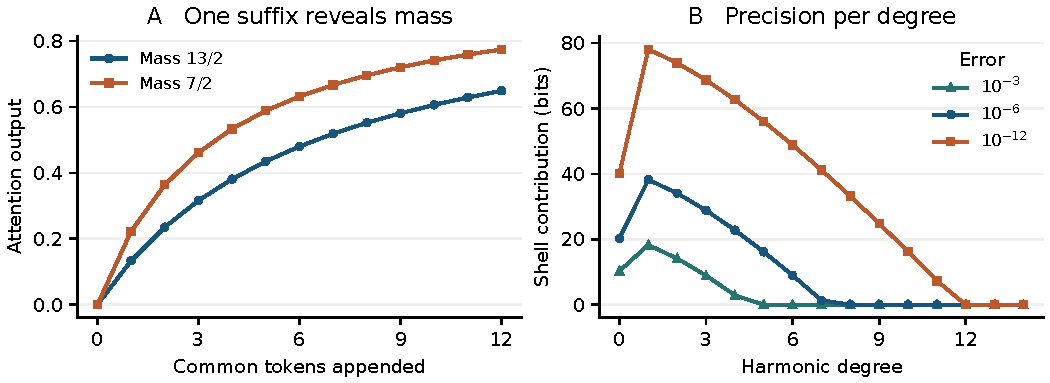
\includegraphics[width=.98\linewidth]{figures/checkpoint.pdf}
\caption{Left: two zero-valued length-four prefixes give different answers after adding the same value-one tokens. At the first append, the gap is $4/45$. Right: the spectral sum underlying the bit proof on the circle at $\beta=1$. Each point is $h_\ell[\log_2(\lambda_\ell/\eps)]_+$ for one scalar channel, before the lower-order covering terms. The vertical scale gives contributions to that sum.}\label{fig:witness}
\end{figure}

\paragraph{Why the bit constant has a factorial $d!$.}
Let $h_\ell$ count the degree-$\ell$ spherical harmonics. There are about $2m^{d-1}/(d-1)!$ modes through degree $m$. Their exponential-kernel eigenvalues satisfy $\log\lambda_\ell=-\ell\log\ell+O_{d,\beta}(\ell+1)$ for $\ell\ge1$. For the upper bound, encode the normalized historical mass and numerator in harmonics. High degrees have small amplitude even when the history is arbitrarily long. Quantizing each coefficient to an absolute tolerance determined by $\eps$ gives a bit cost governed by
\[
  \frac{c}{\log 2}\sum_{\ell} h_\ell[T+\log\lambda_\ell]_+ .
\]
For the converse, length-matched positive and negative suffixes distinguish mass and numerator with stable constants. Independent bounded perturbations to the key density and to each value density then produce a full harmonic ellipsoid of observable prefixes. A packing of the ellipsoid can be realized by ordinary tokens of one common length, even with identical keys in the free-key experiment. Integrating the fraction $1-\ell/m_T$ of significant precision across retained modes gives $1/d$. Appendix~\ref{app:entropy} proves the covering and packing bounds with the same leading constant.

\paragraph{Why the streaming dimension has a different proof.}
Positive polynomial approximations to the kernel yield a recurrent moment matrix. Degree $m$ suffices when the upper Poisson tail at mean $2\beta$ is sufficiently small. For the lower bound, weighted spherical designs put independent mass and value signals in low harmonics. Realizing those weights continuously by fixed-length ordinary token streams makes Borsuk--Ulam applicable to any continuous encoder. Its colliding antipodes admit a separating common suffix. Appendix~\ref{sec:finite} gives the finite inequalities, construction and limiting argument. For instance, with $d=3$, $p=2$, $\beta=1$ and $\eps=10^{-6}$ they certify $74\le r_*(\eps)\le588$. The exact finite optimum is open even in this example.

\section{What keeping exact keys buys in a finite cache}\label{sec:kv}
The free-key theorem asks what remains chargeable once keys are known. A real codec that chooses exact keys must pay to store them. It does gain a precise local certificate: at common queries, keys, masks and gates, the attention probabilities are identical in exact arithmetic. Only value residuals enter the ideal projected difference. Let $a_{hi}$ be the probability at visible position $i$ for query head $h$, $g(h)$ its KV group, $s_{hc}$ a fixed channel gate, and $W$ the output projection. If $|e_{gic}|\le\eta_{gic}$, the sharp worst-case projected $\ell_\infty$ error is
\begin{equation}
 \max_j\sum_{g,i,c}\eta_{gic}\left|\sum_{h:g(h)=g} W_{j,hc}s_{hc} a_{hi}\right| .
 \label{eq:localbody}
\end{equation}
Heads in one group share an error variable. One can attain the radius by choosing its sign from a maximizing combined row. Two heads with equal probabilities, gates one and opposing projections cancel exactly. If $|s_{hc}|\le1$ and every tolerance is at most $\eta$, the radius is at most $\eta\|W\|_{\infty\to\infty}$. Appendix~\ref{app:math} gives the proof, an exact characterization of invisible residuals with affine scores and the additional stability assumptions required to protect a greedy token.

\paragraph{Deployed representation.}
In Qwen3.5-0.8B, 18 recurrent layers and six full-attention layers share the decoding loop \cite{qwen,gdn}. The tested attention reader stores a 256-coordinate BF16 key row in 384 bytes when its exponent range fits, otherwise 512. A value row uses 352 bytes when reconstruction passes its absolute budget and 512 otherwise. The implementation chooses a tolerance just below $1/(128\|W\|_{\infty\to\infty})$ in each layer. Two four-byte headers bring the minimum K/V pair to 744 bytes; a raw key adds 128 and a raw value adds 160. In a packed prefix the encoder pays for the selected modes. For each future token the allocator reserves full-width slots over six layers and two groups: 12,384 bytes, compared with 12,288 in dense BF16. The output error $1/128$ concerns the ideal projection at fixed inputs. Kernel rounding and changes in hidden state have separate effects.

\begin{table}[t]\centering\small
\caption{BF16 Qwen3.5-0.8B on one RTX PRO 6000 Blackwell. For each prefix length, each backend generated 64 tokens in four runs on each of two books. Rates pool tokens divided by elapsed seconds. The final column spans the two observed KV reservations.}\label{tab:rates}
\begin{tabular}{rrrrr}\toprule Prefix (tokens)&Dense (tok/s)&Compact (tok/s)&Change (\%)&Saved (MiB)\\\midrule
\PooledRows\bottomrule\end{tabular}
\end{table}

\paragraph{A whole-model measurement.}
The baseline is dense FlashInfer \cite{flashinfer}. Both paths share projections, recurrent updates and greedy selection. Batch size is one. We take three nested prefixes from each of \emph{Emma} and \emph{Moby-Dick} \cite{nltk}. A warm-up precedes four pairs with alternating order. Timed steps include appending a new K/V record and returning its token ID to Python. All 384 positions in the six distinct continuations match. Pooled throughput varies by less than one percent in either direction (Table~\ref{tab:rates}); the 24 individual timing pairs appear in Appendix~\ref{app:record}. At 131,072 tokens the cache saves 331.1--334.0 MiB. Converting the prefix takes 14.93--15.94 seconds once, which raises the reconstructed single-request total from about 10 seconds to 24.94--25.93 (Figure~\ref{fig:budget}). The reported storage excludes weights, recurrent states and workspace. The six continuations quantify observed agreement; subsequent queries and gates in an autoregressive run need not coincide.

\begin{figure}[t]\centering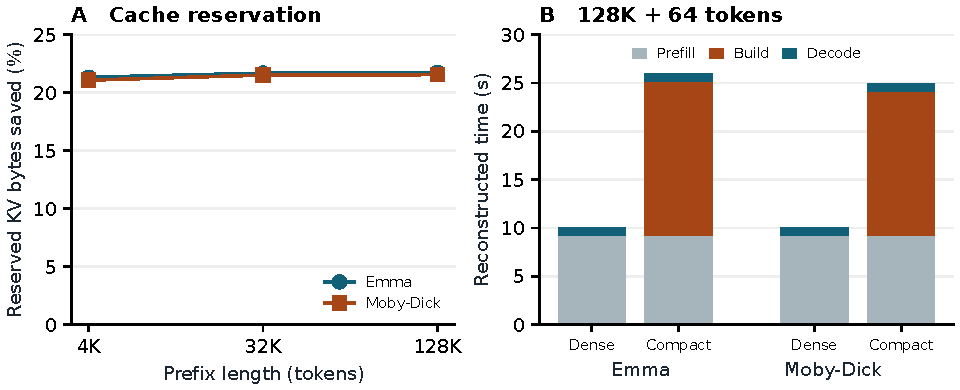
\includegraphics[width=.95\linewidth]{figures/budget.pdf}
\caption{Prefix packing saves KV capacity across the six conditions. At 128K the right panel separates common prefill, cache construction and 64 warm generation steps. Host conversion and kernel preflight are included in the measured compact build.}\label{fig:budget}
\end{figure}

\section{When every recurrent word must survive}\label{sec:word}
A bitwise restart requires the inverse codec to return exactly the original words. If the remaining machine state, arithmetic and inputs are identical, determinism then preserves all later native transitions by induction. Small approximation error alone gives no compression guarantee for this contract. For example, set $X_{ij}=1+2^{-23}d_{ij}$ with $0\le d_{ij}<2^s$, $s\le23$. These positive FP32 matrices lie within relative squared Frobenius error $((2^s-1)2^{-23})^2$ of the all-ones rank-one matrix. They still contain $s$ freely chosen bits per entry (Appendix~\ref{app:words}).

\paragraph{A lower bound that can guide an encoder.}
Consider a row of 128 binary32 words. Within sixteen groups of eight, encode the 31-bit magnitude $a_i$ relative to an integer reference $t$, using a common width per group and a separate sign stream. For $\mathrm{zz}(z)=2z$ for $z\ge0$ and $-2z-1$ otherwise, the width is the bit length of the largest ZigZag residual. If group extrema are $l_j,h_j$, width at most $w\ge1$ is equivalent to
\[
  h_j-2^{w-1}+1\ \le t\le\ l_j+2^{w-1}.
\]
Width zero gives a singleton for a constant group. Each width threshold therefore contributes a known saving over an interval. Sweeping their weighted endpoints yields a global optimum, including byte rounding and ties. With $s$ sign-exception masks, let $R_0,R_*$ be baseline and optimal residual record lengths, and $A$ the cheapest alternative (raw, exponent or zero). The complete record gains exactly $[\min(R_0-R_*,A-R_*)]_+$. Grant each group a distinct free reference and the fixed-header floor becomes
\[
 \min\!\left(A,\,17+4s+\sum_j\left\lceil\log_2(1+h_j-l_j)\right\rceil\right).
\]
Both conclusions apply to an explicit layout. Changing the transform or entropy-coding across rows can cross the floor. Appendix~\ref{app:one} gives the optimization algorithm, a checkable certificate, and an extension to multiple stored references.

\begin{table}[t]\centering\small
\caption{Exact FP32 reconstruction on 2,592 archived heads. Lengths include implemented framing except for the native array. The floor grants free group references with the residual header fixed.}\label{tab:bytes}
\begin{tabular}{@{}lr@{}}\toprule Representation & Total bytes\\\midrule
Dense native words &169,869,312\\
Row modes, midpoint reference &149,047,714\\
Row modes, optimal reference &148,940,720\\
Fixed-header lower bound with free group references &148,335,505\\
Bit shuffle and Zstandard, whole-head frames &142,093,897\\\bottomrule
\end{tabular}
\end{table}

\paragraph{How much of the optimum survives mode selection?}
Three teacher-forced Q4\_0 traces supply all 18 recurrent layers and 16 heads at tokens 1, 428 and 460. This is a separate offline experiment from the BF16 attention run. We serialize and decode every $128\times128$ FP32 head and compare the words. Exact selection saves 2,045,888 candidate bytes, of which 106,994 (5.23\%) survive competition with the other row modes. At aggregate level, even free group references leave 6,241,608 bytes above bit shuffle plus Zstandard (Table~\ref{tab:bytes}). The ordering reverses at each of the two later checkpoints: the optimized local layout is about 0.48--0.59 MB smaller there. The first checkpoint and its equal weight in the census explain the aggregate. A whole-head compressor and a sequential row decoder also expose different access granularities. These figures describe archived words and the specified layouts; they do not measure online recurrent decoding speed.

\paragraph{An implementable consequence of the floor.}
The two frame formats win on different heads. Encode each head both ways, choose the shorter complete frame, and write one selector byte before its existing four-byte length field. An independent pass parses the resulting stream, decodes exactly one selected frame per head, and compares all recovered words against the original. The 2,592-head file occupies \textbf{140,735,906 bytes}, including every selector. It chooses the local format 1,522 times and bit shuffle 1,070 times, improving on always using bit shuffle by 1,357,991 bytes (0.96\%). This gain comes from a change of representation at head granularity. Encoding both candidates incurs extra work. We did not time the selector or test it in a live model. Appendix~\ref{app:mixed} reports the checkpoint breakdown.

\section{Relation to prior work and limits}\label{sec:scope}
Kernel-feature attention stores an unnormalized value sum and a normalizer \cite{kath,schlag}. Streaming attention bounds based on communication reductions, discrepancy, polynomial approximations and partitioning study resource models with explicit bit or stream constraints \cite{haris,balance,chen}. Query-distribution risk supplies another objective \cite{risk}. Our continuous dimension result concerns deterministic uniform accuracy in fixed dimension. The bit theorem charges one message and grants exact suffix storage. It cannot be applied as a constant-memory implementation of repeated finite-precision updates. Work on isotropic kernels already relates spherical spectra to covering numbers \cite{entropy}, while nonlinear widths characterize approximation by continuous parameters \cite{devore}. The extra steps here are to recover both profiles from common continuations and realize a matching packing by valid prefixes.

KIVI quantizes keys and values on different axes \cite{kivi}; bounded-error quantized attention propagates score and value errors \cite{calver}; weighted value projection accounts for attention priorities \cite{salfati}. Equation~\eqref{eq:localbody} takes the support function after grouping the shared variables. Integer frame-of-reference coding, floating-point layouts and bit shuffling provide the coding context for the recurrent experiment \cite{lemire,alp,shuffle}. Its format floor can distinguish an exhausted reference search from a potentially better layout.

The theoretical sphere, arbitrary suffix values, exact arithmetic and asymptotic accuracy do not describe the measured model's reachable states. The empirical evidence covers one GPU session, two books and 64-token continuations for attention, and three traces with three checkpoint positions for recurrent words. No run used both codecs together. Adding their byte percentages would mix distinct denominators, precisions and workloads. Joint deployment would require measuring total peak device memory, prefix reuse, recurrent serialization and the resulting token sequence in one execution. For the existing runs the defensible conclusion is narrower: keeping a normalizer has a quantifiable information price, while a concrete decoder's storage and latency depend on where and how it pays that price.

\paragraph{Reproduction.}
The CPU notebook regenerates the figures from harmonic calculations, one archived GPU trace and a per-head census. It checks exact arithmetic witnesses and re-encodes a portable raw-word subset. The appendix gives the full protocols, resource boundaries and AI-assistance disclosure. The anonymous copy includes the conference checklist.


\begin{thebibliography}{99}
\bibitem{kath} A. Katharopoulos, A. Vyas, N. Pappas and F. Fleuret.
Transformers are RNNs: Fast autoregressive transformers with linear attention. \emph{ICML}, PMLR 119, 5156--5165, 2020.
\bibitem{schlag} I. Schlag, K. Irie and J. Schmidhuber.
Linear transformers are secretly fast weight programmers. \emph{ICML}, PMLR 139, 9355--9366, 2021.
\bibitem{haris} T. Haris and K. Onak.
Compression barriers in autoregressive transformers. \emph{COLT}, PMLR 291, 2757--2785, 2025.
\bibitem{balance} E. Kochetkova, K. J. Sheth, I. Han, A. Zandieh and M. Kapralov.
Streaming attention approximation via discrepancy theory. \emph{Advances in Neural Information Processing Systems} 38, 2025.
\bibitem{chen} J. Y. Chen, Y. Feng, P. Indyk, M. Kapralov, E. Kochetkova and B. Prokhorov.
Towards tight bounds for streaming attention. \href{https://arxiv.org/abs/2606.07205}{arXiv:2606.07205}, 2026.
\bibitem{risk} L. Haverbeck, C. Amo Alonso, A. F. Posada-Moreno, S. Trimpe and M. Pavone.
The risk of KV cache compression. \href{https://arxiv.org/abs/2607.01520}{arXiv:2607.01520v2}, 2026.
\bibitem{entropy} K. Gonzalez and T. Jord\~ao. A close look at the entropy numbers of the unit ball of the reproducing Hilbert space of isotropic positive definite kernels. \emph{Journal of Mathematical Analysis and Applications}, 534(2), 2024. \url{https://arxiv.org/abs/2304.14103}.
\bibitem{devore} R. A. DeVore, R. Howard and C. A. Micchelli.
Optimal nonlinear approximation. \emph{Manuscripta Mathematica}, 63, 469--478, 1989. \href{https://doi.org/10.1007/BF01171759}{doi:10.1007/BF01171759}.
\bibitem{atkinson} K. Atkinson and W. Han.
\emph{Spherical Harmonics and Approximations on the Unit Sphere: An Introduction}.
Lecture Notes in Mathematics 2044, Springer, 2012. \href{https://doi.org/10.1007/978-3-642-25983-8}{doi:10.1007/978-3-642-25983-8}.
\bibitem{design} A. Bondarenko, D. Radchenko and M. Viazovska.
Optimal asymptotic bounds for spherical designs. \emph{Annals of Mathematics}, 178(2), 443--452, 2013. \href{https://doi.org/10.4007/annals.2013.178.2.2}{doi:10.4007/annals.2013.178.2.2}.
\bibitem{borsuk} J. Matou\v{s}ek. \emph{Using the Borsuk--Ulam Theorem}. Springer, 2003. \href{https://doi.org/10.1007/978-3-540-76649-0}{doi:10.1007/978-3-540-76649-0}.
\bibitem{universal} C. A. Micchelli, Y. Xu and H. Zhang. Universal kernels. \emph{Journal of Machine Learning Research}, 7, 2651--2667, 2006.
\bibitem{kivi} Z. Liu, J. Yuan, H. Jin, S. Zhong, Z. Xu, V. Braverman, B. Chen, and X. Hu. KIVI: A tuning-free asymmetric 2bit quantization for KV cache. \emph{ICML}, PMLR 235, 32332--32344, 2024. \href{https://proceedings.mlr.press/v235/liu24bz.html}{Proceedings}.
\bibitem{calver} D. Calver. Runtime-certified bounded-error quantized attention. \href{https://arxiv.org/abs/2605.20868}{arXiv:2605.20868}, 2026.
\bibitem{salfati} S. Salfati. Attention-weighted value projection for KV-cache compression. \href{https://arxiv.org/abs/2604.11501}{arXiv:2604.11501}, 2026.
\bibitem{flashinfer} Z. Ye, L. Chen, R. Lai, W. Lin, Y. Zhang, S. Wang, T. Chen, B. Kasikci, V. Grover, A. Krishnamurthy, and L. Ceze. FlashInfer: Efficient and customizable attention engine for LLM inference serving. \emph{MLSys}, 7, 2025. \href{https://arxiv.org/abs/2501.01005}{Paper}.
\bibitem{qwen} Qwen Team. \emph{Qwen3.5-0.8B model card and configuration}. 2026. \href{https://huggingface.co/Qwen/Qwen3.5-0.8B/tree/2fc06364715b967f1860aea9cf38778875588b17}{Model repository at the evaluated revision}.
\bibitem{nltk} S. Bird, E. Klein, and E. Loper. \emph{Natural Language Processing with Python}. O'Reilly, 2009. \href{https://www.nltk.org/book/ch02.html}{Chapter 2, accessing text corpora and lexical resources}.
\bibitem{gdn} S. Yang, J. Kautz, and A. Hatamizadeh. Gated Delta Networks: Improving Mamba2 with Delta Rule. \emph{ICLR}, 2025. \url{https://arxiv.org/abs/2412.06464}.
\bibitem{lemire} D. Lemire and L. Boytsov. Decoding billions of integers per second through vectorization. \emph{Software: Practice and Experience}, 45(1), 2015. \url{https://doi.org/10.1002/spe.2203}.
\bibitem{shuffle} K. Masui et al. A compression scheme for radio data in high performance computing. \emph{Astronomy and Computing}, 12, 2015. \url{https://arxiv.org/abs/1503.00638}.
\bibitem{alp} A. Afroozeh, L. X. Kuffo, and P. A. Boncz. ALP: Adaptive lossless floating-point compression. \emph{Proceedings of the ACM on Management of Data}, 2023. Presented at SIGMOD 2024. \url{https://doi.org/10.1145/3626717}.
\bibitem{hitting} C. Chung, A. Vigneron, and H.-K. Ahn. Maximum coverage by $k$ lines. \emph{Symmetry}, 16(2), 206, 2024. See Section 6 on partial interval hitting. \url{https://doi.org/10.3390/sym16020206}.
\bibitem{archive} Local exact GDN state fusion and native Qwen recurrent-state captures. Research artifacts, October--November 2026. Source archive names, selected native words, codec and measurement records are described in Appendix~\ref{app:experiment} and the accompanying reproducibility material.
\end{thebibliography}

\clearpage
\fi
\appendix
\section{The bit cost of a single checkpoint}\label{app:entropy}
We prove the bit law independently of the streaming dimension converse. Fix $d\ge2$, $p\ge1$ and $\beta>0$. Use normalized surface measure $\omega$ on $\mathbb S^{d-1}$. A nonempty prefix of known length $n$ defines the empirical probability $\mu=n^{-1}\sum_i\delta_{k_i}$ and vector measure $\nu=n^{-1}\sum_i v_i\delta_{k_i}$, with $\|v_i\|_2\le1$. Their spherical exponential transforms are $z$ and $x$, so $e^{-\beta}\le z\le e^\beta$ and $\|x\|_2\le z$. At a checkpoint the encoder sees the whole prefix and sends one fixed-width message. The decoder subsequently receives the entire exact suffix, and can use arbitrary working storage and exact arithmetic after the cut. Its worst-case Euclidean read error is at most $\eps$ at every requested query, including after an empty suffix. Define $\Bchk$ as the supremum, over $n$, of the least required number of bits for that $n$. Encoders and decoders may depend on $n$. In $\Bfree$ the ordered prefix keys are also available to the decoder; their transmission cost is excluded. There is no continuity assumption on a finite-message encoder.

\begin{theorem}[Entropy of resumable spherical attention]\label{th:bits}
Set $T=\log(1/\eps)$ and $m_T=T/\log T$. Then
\[
 \lim_{\eps\downarrow0}\frac{\Bchk(\eps)}{T m_T^{\,d-1}}
 =\frac{2(p+1)}{d!\log2},
 \qquad
 \lim_{\eps\downarrow0}\frac{\Bfree(\eps)}{T m_T^{\,d-1}}
 =\frac{2p}{d!\log2}.
\]
The same limits hold with supplied global rotations of the existing keys and a fixed continuous orthogonal action on the values.
\end{theorem}

\subsection{Which metric does a future read observe?}
Let $F(P,P')$ be the supremum of the Euclidean output gap over all common suffixes and final queries of two length-$n$ prefixes. Write $u=\sup_q|z-z'|$ and $v=\sup_q\|x-x'\|_2$. All transforms in this section use per-prefix averages. Adding exact suffix sums divided by $n$ changes neither profile difference. Normalizing the two totals gives $F\le e^\beta(u+v)$, since each total mass is at least $e^{-\beta}$ and each exact read has norm at most one. In the presence of rotations the prefix functions are composed with a common orthogonal change of argument and the numerator is rotated; the suprema are invariant.

For the reverse comparison fix $q$ and put $b=e^\beta$. Append $n$ copies of key $q$ carrying $+e$ or $-e$, for a fixed unit vector $e$. Write $s=z/b$, $a=x/b$. The two outputs are $y_\pm=(a\pm e)/(1+s)$, with $s\le1$. Their half-difference is $e/(1+s)$ and their mean is $a/(1+s)$. If the two prefixes' responses on each probe differ by at most $F$, both the mean and the half-difference differ by at most $F$. Thus $|s-s'|\le4F$ and $\|a-a'\|_2\le 2F+4F=6F$, since the mean has norm at most one. In particular
\begin{equation}
 \| (z-z',x-x')\|_{L^2(\omega;\mathbb R^{p+1})}\le 8e^\beta F(P,P').
 \label{eq:inverse}
\end{equation}
The identities apply equally to ideal probability and vector measures, interpreted with probe mass $b$. All constants are independent of $n$. Any two ordinary prefixes assigned the same message must satisfy $F\le2\eps$. The free-key version uses this statement only for pairs with identical keys.

\subsection{Harmonic scales}
Let $h_\ell$ be the dimension of degree-$\ell$ spherical harmonics and $D_m=\sum_{\ell\le m}h_\ell$. In a real orthonormal basis, $\sum_jY_{\ell j}(q)^2=h_\ell$ by rotational invariance and integration. The spherical convolution with $e^{\beta q^\top k}$ acts as a scalar $\lambda_\ell$ at each degree. The moment tensor calculation in Lemma~\ref{lem:spectral} applies with continuous surface measure: each term $(q^\top k)^j$ acts by a nonnegative scalar, vanishes on degrees above $j$, and at $j=\ell$ contributes $\ell!/[d(d+2)\cdots(d+2\ell-2)]$ before exponential weighting. For the upper estimate, deleting the Taylor terms below $\ell$ leaves the same operator on degree $\ell$. Its norm is bounded by the supremum of the absolute kernel remainder (probability measure), giving
\[
 \frac{\beta^\ell}{d(d+2)\cdots(d+2\ell-2)}\le \lambda_\ell
 \le e^\beta\frac{\beta^\ell}{\ell!},\qquad
 \log\lambda_\ell=-\ell\log(\ell\vee1)+O_{d,\beta}(\ell+1).
\]
These inequalities include degree zero with the empty product. An empirical profile has coefficient $\lambda_\ell\int Y_{\ell j}\,d\mu$ or $\lambda_\ell\int Y_{\ell j}\,d\nu_c$. The whole degree block of each scalar profile before multiplication by $\lambda_\ell$ has Euclidean norm at most $\sqrt{h_\ell}$ by the addition identity and total variation at most one. At every query the norm of the corresponding degree contribution to a scalar channel is consequently at most $h_\ell\lambda_\ell$. Absolute uniform summability follows from the factorial bound. Completeness of spherical harmonics identifies the series with the original continuous profile.

\paragraph{A sum used in both bounds.}
Let $c$ be a fixed number of scalar channels, and define $[t]_+=\max(0,t)$. For any fixed $K>1$,
\begin{equation}
 \sum_{\ell\le K m_T} c h_\ell[T+\log\lambda_\ell]_+
 \sim \frac{2c}{d!}\,T m_T^{d-1}. \label{eq:shellsum}
\end{equation}
Replacing the bracket argument by $T-\ell\log(\ell\vee1)$ costs $O(m_T^{d})=o(Tm_T^{d-1})$, since $[\,\cdot\,]_+$ is 1-Lipschitz. Uniformly for $0\le\ell\le K m_T$, $\ell\log(\ell\vee1)/T=\ell/m_T+o(1)$; this follows from $\log m_T/\log T\to1$ and boundedness of $s\log s$ on $[0,K]$. The exact dimension formula in Section~\ref{sec:upper} gives $h_\ell\sim2\ell^{d-2}/(d-2)!$ (on the circle $h_\ell=2$ for $\ell\ge1$). The normalized sum tends to $2c/(d-2)!\int_0^1 s^{d-2}(1-s)\,ds=2c/d!$. A uniform additive $O(\log(m_T+2))$ inside the brackets changes only lower-order terms. Discarding one constant coefficient costs $O(T)$, also lower order since $d\ge2$.

\subsection{Upper bound by quantizing a checkpoint once}
Take $m=\lceil 2m_T\rceil$ and $c=p+1$ for the joint code, or $c=p$ for free keys. The tail bound $\sum_{\ell>m}h_\ell e^\beta\beta^\ell/\ell!=\exp[-m\log m+O_{d,\beta}(m)]=o(\eps)$ holds as an upper estimate. For each of the $c$ scalar profiles, round every retained coefficient to the nearest multiple of
\[
 \Delta=\frac{\eps e^{-\beta}}{32\sqrt{p+1}\,(D_m+1)^2}.
\]
Summing the absolute coefficient errors against the basis at a query costs at most $\Delta\sum_{\ell\le m}h_\ell\sqrt{h_\ell}\le \Delta D_m^2$ per channel. For sufficiently small $\eps$, the combined uniform error of the scalar mass and the vector numerator is therefore below $\eps e^{-\beta}/4$ each. Free keys give the mass exactly. For an exact suffix, the decoded denominator is at least $e^{-\beta}(1-\eps/4)$, in units of prefix length. The normalized read differs by at most $(\eps/2)/(1-\eps/4)\le\eps$ for $\eps\le1$. Multiplication by $n$ restores the actual scale if raw suffix sums are used. Future rotations can be applied by rotating the query back to the checkpoint frame and rotating the predicted vector forward; this introduces no further quantization.

Each scalar coefficient lies in $[-\sqrt{h_\ell}\lambda_\ell,\sqrt{h_\ell}\lambda_\ell]$. The number of rounding outcomes per coordinate is at most $2+2\sqrt{h_\ell}\lambda_\ell/\Delta$. An index into their Cartesian product requires the ceiling of its base-two logarithm. Its natural logarithm is bounded by
\[
 \sum_{\ell\le m} c h_\ell [T+\log\lambda_\ell]_+ + O_{d,p,\beta}(D_m\log(m+2)).
\]
The last term includes levels with only one or two rounding outcomes. Equation~\eqref{eq:shellsum} and conversion to bits prove the limsup. Computation of the coefficients is unrestricted at the cut; the argument charges a single message.

\subsection{Lower bound from profiles attainable by ordinary tokens}
Choose real polynomials $u,f_1,\ldots,f_p$ of degree at most $m$, with the constant coefficient of $u$ deleted. Their joint coefficient vector ranges over the Euclidean unit ball. Put $\alpha=(2\sqrt{D_m})^{-1}$. Against $\omega$ take key density $1+\alpha u$ and conditional value vector $\alpha f/(1+\alpha u)$. The key density integrates to one and is at least $1/2$. The evaluation-vector identity through degree $m$ gives $\|f(q)\|_2\le\sqrt{D_m}$ and $|u(q)|\le\sqrt{D_m}$, so the conditional values are legal. Subtract the unperturbed profile. In the joint $L^2$ norm, the resulting profile vectors fill an ellipsoid with semiaxes $\alpha\lambda_\ell$, one for every retained coefficient. With free keys take $u=0$ throughout, keep only the $p$ value channels and use the same uniform key measure for all parameters.

Set $m=\lceil2m_T\rceil$ and $r=64 e^\beta\eps$. Restrict to axes longer than $r$. A maximal $r$-separated set in the resulting ellipsoid covers it with radius-$r$ Euclidean balls. Comparing volumes gives at least $\prod_i (\alpha\lambda_{\ell(i)}/r)$ centers, with the product restricted to these axes. This finite set suffices. Its ideal prefixes can be approximated by ordinary equal-length prefixes with joint profile error below $r/8$ for every center. To see this, partition the sphere into finitely many Borel cells of small diameter. For each center put its key mass in each cell at one representative key, using its mass-weighted mean value in that cell. Uniform continuity of the kernel bounds the two transform errors uniformly in $q$. Round the resulting weights to multiples of $1/n$ with total one; for $H$ cells their total absolute rounding error is at most $2H/n$. The same large $n$ works for all centers. In the free-key case the cell weights, rounded counts and key order can be chosen identical because all key marginals coincide. Values remain in the unit ball. This construction only has to realize finitely many points; the continuous family needed for the streaming theorem is constructed separately in Lemma~\ref{lem:realize}.

The realized profiles are at least $3r/4$ apart. A shared message would instead put them within $16 e^\beta\eps$ by \eqref{eq:inverse}. All centers require different messages, including with free keys in the fixed-key construction. Taking natural logarithms yields
\[
 \sum_{\ell\le m}c h_\ell[T+\log\lambda_\ell+\log\alpha-\log(64e^\beta)]_+-O(T).
\]
The subtracted term allows for the fixed scalar mass coefficient. Since $\log\alpha=O(\log(m+2))$, \eqref{eq:shellsum} gives the matching liminf after division by $\log 2$. This completes Theorem~\ref{th:bits}.

\paragraph{Reading the coefficient.}
Relative to the continuous streaming dimension $r_*(\eps)$, the joint one-checkpoint bit cost is asymptotic to $T r_*(\eps)/(d\log2)$. Successively higher degrees have fewer significant digits. This accounts for the factor $1/d$ compared with assigning $T/\log 2$ bits to every retained real coordinate. The upper bound performs only one rounding of the historical contribution. Repeated rounding after each token, a private or unknown prefix length, bounded decoder workspace, a fixed deployment horizon and exact IEEE-word restart each define other coding problems.


\section{Finite bounds and proofs}\label{sec:finite}
Let $d\ge2$, $p\ge1$ and $\beta>0$ be fixed. The target is the normalized exponential-weighted mean on $\Sphere$ with values in $\Ball$. The budget $r_*$ counts persistent real coordinates of a deterministic encoder that is continuous on each fixed-length prefix. The budget $\rf$ supplies the key and rotation history for free. All accuracy statements below use the Euclidean norm, all finite histories and independently chosen queries. This section proves both continuous-state constants. It also gives an exact converse at zero error.

For $L\ge1$ let $D=D_{d,L}$ be the dimension of spherical polynomials of degree at most $L$. Define
\begin{align}
 c_{d,0}&=1, &
 c_{d,\ell}&=\frac{\beta^\ell}{d(d+2)\cdots(d+2\ell-2)}\quad(\ell\ge1),&
 \low&=\min\{1,c_{d,L}\}.\label{eq:spectralconst}
\end{align}
For $m\ge0$ put $\delta_m=\Pr\{\operatorname{Poisson}(2\beta)>m\}$.

\begin{theorem}[Finite inequalities]\label{thm:finite}
For every $m\ge0$ and $L\ge1$ the following implications hold.
\begin{align}
 2\delta_m/(1-\delta_m)\le\eps
 &\ \Longrightarrow\ r_*(\eps)\le(p+1)D_{d,m},\label{eq:upper}\\
 \eps<e^{-3\beta}\low/(8\sqrt D)
 &\ \Longrightarrow\ r_*(\eps)\ge(p+1)D-1,\label{eq:lower}\\
 \delta_m\le\eps
 &\ \Longrightarrow\ \rf(\eps)\le pD_{d,m},\label{eq:freeup}\\
 \eps<e^{-\beta}\low/(2\sqrt D)
 &\ \Longrightarrow\ \rf(\eps)\ge pD.\label{eq:freelow}
\end{align}
The lower bounds use identity rotations. The upper bounds allow any supplied rotations and any fixed continuous orthogonal representation on values.
\end{theorem}

\subsection{Positive polynomial moments}\label{sec:upper}
Set $P_m(t)=e^{-\beta}\sum_{a=0}^m [\beta(1+t)]^a/a!$. For $-1\le t\le1$, the ratio $P_m(t)/e^{\beta t}$ equals the probability that a Poisson variable of mean $\beta(1+t)$ is at most $m$. Hence $1-\delta_m\le P_m(t)/e^{\beta t}\le1$. If $\widetilde Z,\widetilde N$ are the two sums computed with $P_m$, then
\begin{equation}
 |Z-\widetilde Z|\le\delta_m Z,\qquad
 \norm{N-\widetilde N}_2\le\delta_m Z,\qquad
 \widetilde Z\ge(1-\delta_m)Z>0.\label{eq:uniform}
\end{equation}
Writing the difference of normalized outputs over $\widetilde Z$, and using $\norm{N/Z}_2\le1$, proves the error in \eqref{eq:upper}. Replacing $\widetilde Z$ by $Z$ proves the error in \eqref{eq:freeup}.

Use probability surface measure $\omega$. Choose real orthonormal spherical harmonics through degree $m$, concatenate them into a column $Y(k)$ and put $w(v)=(1,v^\top)^\top$. Harmonic decomposition of homogeneous polynomials gives
\[
 D_{d,m}=\binom{m+d-1}{d-1}+\binom{m+d-2}{d-1}.
\]
Indeed, the degree-$\ell$ harmonic dimension is the difference between the dimensions of homogeneous polynomials of degrees $\ell$ and $\ell-2$, with negative degrees empty. Summation telescopes \cite{atkinson}. For each $q$, the function $k\mapsto P_m(\ang qk)$ has expansion $a(q)^\top Y(k)$ in that basis. The moment matrix
$M=\sum_iY(k_i)w(v_i)^\top$ recovers both sums via $a(q)^\top M$. For a rotation $R$, write $Y(Rk)=U(R)Y(k)$ and $B(R)=\operatorname{diag}(1,\rho(R))$. The update is
\begin{equation}
 M_{t}=U(R_t) M_{t-1} B(R_t)^\top+Y(k_t)w(v_t)^\top,\qquad M_0=0.
 \label{eq:update}
\end{equation}
Each finite-prefix state map is continuous. The frame is already incorporated in $M_t$. There are $(p+1)D_{d,m}$ entries, or $pD_{d,m}$ if the mass is computed from free keys. For a nonnegative integer Poisson variable $X$ of mean $2\beta$,
$\mathbf1_{X\ge m+1}\le\binom{X}{m+1}$ and hence $\delta_m\le(2\beta)^{m+1}/(m+1)!$.

\subsection{A spectral estimate on a finite design}\label{sec:spectral}
Fix a spherical $2L$-design $x_1,\ldots,x_H$ with equal weights. Existence follows from \cite{design}. On the circle a regular polygon with more than $2L$ vertices suffices. Let $V_{ia}=Y_a(x_i)$ for the harmonics through degree $L$. Design exactness applied to products gives $V^\top V/H=I_D$. Rotation invariance makes $\sum_aY_a(x)^2$ constant, and its integral is $D$. Thus $\norm{Y(x)}_2=\sqrt D$. On grid vectors use $\ang fg_H=H^{-1}\sum_i f_i g_i$ and let $K_{ji}=H^{-1}\K(x_j,x_i)$.

\begin{lemma}[Visible low degrees]\label{lem:spectral}
If $g$ is in the column space of $V$, then $\norm{Kg}_H\ge\low\norm g_H$. The squared bounds add across vector components.
\end{lemma}
\begin{proof}
First truncate the exponential at degree $L$ in the unshifted variable. For each $a$, the kernel $(x^\top y)^a$ is positive semidefinite since it is the inner product of $x^{\otimes a}$ and $y^{\otimes a}$. The omitted exponential tail is therefore a positive semidefinite matrix on the grid, by convergence of finite sums.

For a harmonic homogeneous polynomial $h_\ell$ of degree $\ell\le L$, design integration of $(x^\top y)^a h_\ell(y)$ is exact for $a\le L$. Its sphere integral is a scalar multiple of $h_\ell(x)$ on $\Sphere$. To see both the sign and normalization, represent $h_\ell$ by a symmetric trace-free tensor. The degree-$2j$ moment of a uniform point $y$ is the sum of all Kronecker-delta pairings divided by $d(d+2)\cdots(d+2j-2)$. Odd moments vanish. This follows by writing a standard Gaussian as its independent radius and uniform direction, expanding its moment generating function, and using $\mathbb E\norm G^{2j}=d(d+2)\cdots(d+2j-2)$. A pairing of two tensor indices of $h_\ell$ vanishes by tracelessness. Each surviving term contracts all $\ell$ indices with copies of $x$ and pairs the remaining copies among themselves. Its value is $h_\ell(x)\norm x^{a-\ell}$, with a positive prefactor. At $a=\ell$ there are exactly $\ell!$ surviving pairings. The degree-zero calculation uses the empty product.

After multiplication by $\beta^a/a!$, the truncated kernel therefore has eigenvalue at least $c_{d,\ell}$ on the sampled degree-$\ell$ harmonics. These spaces are orthogonal in the grid norm. The ratio $c_{d,\ell+1}/c_{d,\ell}=\beta/(d+2\ell)$ decreases in $\ell$, so the minimum through degree $L$ is attained at an endpoint. Adding the positive semidefinite tail gives $\ang{g}{Kg}_H\ge\low\norm g_H^2$ on the sampled subspace. Cauchy--Schwarz gives the stated norm inequality even if $Kg$ leaves that subspace.
\end{proof}

\subsection{Independent mass and value perturbations}\label{sec:perturb}
Choose a scalar spherical polynomial $u$ with zero constant harmonic coefficient and $p$ spherical polynomials $f=(f_1,\ldots,f_p)$ allowing constants, all of degree at most $L$. The combined vector of coefficients $\theta$ ranges over the Euclidean unit sphere in $\R^M$, where $M=(p+1)D-1$. Write $u_i=u(x_i)$, $f_i=f(x_i)$ and $a=1/(2\sqrt D)$. Isometry on the design gives $\norm u_H^2+\sum_j\norm{f_j}_H^2=1$. Pointwise, $|u_i|\le\sqrt D$ and $\norm{f_i}_2\le\sqrt D$. Form a weighted prefix
\begin{equation}
 w_i=(1+a u_i)/H,\qquad v_i= a f_i/(1+a u_i).
 \label{eq:weights}
\end{equation}
The weights sum to one and are strictly positive. Values lie in the unit ball. At a grid query the antipodal prefixes have masses $d_0\pm z$ and numerators $\pm X$, where $d_0=(K\mathbf1)_j$, $z=a(Ku)_j$, and $X=a(Kf)_j$. By Lemma~\ref{lem:spectral} and averaging, some $j$ satisfies
\begin{equation}
 z^2+\norm X_2^2\ge a^2\low^2.\label{eq:signal}
\end{equation}

Fix a unit vector $e\in\R^p$ and a suffix key $k_*$ in advance. At the selected query let $b=\K(x_j,k_*)$ and $A=d_0+b$. Each choice of sign specifies a common suffix for the antipodal pair. For the resulting differences $\Delta_\sigma$ of the two outputs,
\begin{align}
 \Delta_\sigma&=\frac{X+\sigma be}{A+z}-\frac{-X+\sigma be}{A-z}
 =\frac{2(AX-\sigma bze)}{A^2-z^2},\nonumber\\
 \max_{\sigma=\pm1}\norm{\Delta_\sigma}_2
 &\ge \frac{2\sqrt{A^2\norm X_2^2+b^2z^2}}{A^2-z^2}
 \ge \frac{e^{-3\beta}}2\sqrt{\norm X_2^2+z^2}.
 \label{eq:twosigns}
\end{align}
The first inequality is the root-mean-square bound over the signs. The second uses $0<b\le A\le 2e^\beta$, $b\ge e^{-\beta}$ and $A>|z|$. Consequently the ideal separation for some query and sign is at least $g=e^{-3\beta}\low/(4\sqrt D)$.

\subsection{Fixed-length realization by ordinary tokens}\label{sec:realization}
\begin{lemma}[Uniform continuous realization]\label{lem:realize}
Let a compact parameter space index finitely many fixed keys on a path-connected sphere, strictly positive continuous weights summing to one and continuous values in $\Ball$. For every $\eta>0$ there is a single integer $n$ and a continuous map from the parameter space to $n$ ordinary key--value tokens, whose normalized mass and numerator sums approximate the weighted profiles within $\eta$ at every query.
\end{lemma}
\begin{proof}
Choose fixed continuous arcs joining consecutive keys in a cycle. Assign total time $1-\tau$ to plateaus and $\tau$ to the arcs, with plateau $i$ of duration $(1-\tau)w_i(\theta)$ and each arc of duration $\tau/H$. On a plateau keep the key and value fixed, and on an arc interpolate its endpoint values linearly. Compactness and positivity bound plateau durations away from zero. The pieces match at moving endpoints, giving a jointly continuous path $(k_\theta(s),v_\theta(s))$ on the compact product of parameters and $[0,1]$. For the scalar and vector integrands $\K(q,k_\theta(s))$ and $\K(q,k_\theta(s))v_\theta(s)$, the plateau contribution is exactly $1-\tau$ times the required weighted profile. The integral differs from the target by at most $2\tau e^\beta$ in either norm. Choose $\tau$ to make this less than $\eta/2$.

Uniform continuity jointly in $s,\theta,q$ then gives an equal-step midpoint Riemann sum of error less than $\eta/2$ for one $n$, simultaneously for all parameters and queries. The $n$ midpoint samples have unit token weight, normalized by $n$ in the comparison. Each sample depends continuously on $\theta$. Prefix queries and rotations may be fixed independently of the parameter.
\end{proof}

\paragraph{From a collision to a contradiction.}
Assume $2\eps<g$ and choose $\eta$ so that $g-2\eta e^\beta>2\eps$. Apply Lemma~\ref{lem:realize} to \eqref{eq:weights}. If $r<M$, the realized prefix state is a continuous map $S^{M-1}\to\R^r$. By Borsuk--Ulam \cite{borsuk}, padding the codomain with zeros if needed, some antipodal parameters have the same state. Choose their distinguishing design query and sign. Append $n$ copies of $k_*$ carrying the common value $\sigma e$, with identity rotations, fixed intermediate queries and the selected final query. Dividing the two prefix and suffix sums by $n$ makes the suffix mass exactly $b$. For each of the two prefixes the realized output differs from its ideal one by at most $\eta e^\beta$: the total denominator is at least $2e^{-\beta}$, the ideal output norm is at most one, and the two profile errors are each at most $\eta$. The realized outputs are thus separated by more than $2\eps$. The identical states and identical future force identical predictions, contradicting the triangle inequality. This proves \eqref{eq:lower}. The length is chosen before the collision. The query and sign are chosen afterward.

\paragraph{An explicit sufficient horizon.}
For the spherical construction, choose arcs of length at most $\pi$. The scalar integrand on each arc has total variation at most $\pi\beta e^\beta$, uniformly in $q$. The vector integrand has variation at most $e^\beta(\pi\beta+2)$ by the product rule for variation, since a straight segment between values has length at most two. Plateaus add zero variation. For any continuous vector-valued path of total variation $V$, the norm of the midpoint quadrature error is at most $V/n$: bound the error on each subinterval by its length times its variation and sum. Thus either profile error is at most
\[
 2\tau e^\beta+H e^\beta(\pi\beta+2)/n.
\]
With $\eta=(g-2\eps)e^{-\beta}/4$, any $0<\tau\le\min\{1/2,\eta/(4e^\beta)\}$ and $n\ge 2H e^\beta(\pi\beta+2)/\eta$ suffice. This gives a finite counterexample of at most $2n$ tokens for every encoder excluded by \eqref{eq:lower}, with $n$ chosen as the ceiling of the displayed threshold. The design, arc paths and length can all be fixed before examining the encoder.

\paragraph{The free-key converse.}
Use the same design, with its $H$ ordinary keys in a fixed order, each once, and set $v_i=f(x_i)/\sqrt D$. Here all $pD$ coefficients of the vector polynomial $f$ lie on their unit sphere, and $\norm{v_i}_2\le1$. For $r<pD$ some antipodal pair has identical paid state. The key-only history is identical as well. Lemma~\ref{lem:spectral} gives a grid query with $\norm{(Kf)_j}_2\ge\low$. Append $H$ copies of the same key with zero value and read that query. The two exact outputs differ by
$2\norm{(Kf)_j}_2/(\sqrt D\,(d_0+b))\ge e^{-\beta}\low/\sqrt D$.
This contradicts accuracy when the strict inequality in \eqref{eq:freelow} holds. The suffix permits the final query to be selected after the prefix collision even in an update-then-read implementation.

\subsection{Asymptotic inversion}\label{sec:limit}
The product in \eqref{eq:spectralconst} is $2^L\Gamma(L+d/2)/\Gamma(d/2)$. Stirling's formula gives
\[
 \log\!\left(\frac{8e^{3\beta}\sqrt{D_{d,L}}}{\lambda_{d,L}}\right)
 =L\log L+O_{d,\beta}(L).
\]
The free-key threshold has the same leading logarithm. For fixed $0<u<1$ and $T=\log(1/\eps)$ take $L=\lfloor(1-u)T/\log T\rfloor$. Then $L\log L=(1-u+o(1))T$, activating both lower bounds for small $\eps$. For $m=\lceil(1+u)T/\log T\rceil$ the factorial upper bound on $\delta_m$ gives $\log\delta_m\le-(1+u+o(1))T$. Both upper bounds apply. Dividing by $(T/\log T)^{d-1}$ and using $D_{d,L}\sim2L^{d-1}/(d-1)!$ puts the liminf and limsup between the corresponding multiples of $(1-u)^{d-1}$ and $(1+u)^{d-1}$. Sending $u$ to zero proves both limits.

\section{Exact future equivalence}\label{sec:exact}
For a finite prefix in its current frame let $\mu=\sum_i\delta_{k_i}$ and $\nu=\sum_i v_i\delta_{k_i}$, the latter a vector measure. For each $q$, append the same key of known weight $b>0$ and use values $0$ and $e$ in two separate tests. If outputs agree between prefixes on both tests, the difference $be/(Z+b)$ agrees between them. It determines $Z$ and then $N$ at that query. Equality of future readouts therefore implies equality of all exponential transforms of $\mu$ and each coordinate of $\nu$.

Here is a finite-support injectivity proof. If a signed difference $\xi=\sum_{i=1}^J c_i\delta_{x_i}$ at distinct $x_i$ has identically zero transform, integrate its transform against $\xi$. Absolute convergence permits the expansion
\begin{equation}
 0=\sum_{i,j}c_i c_j e^{\beta\ang{x_i}{x_j}}
 =\sum_{a=0}^{\infty}\frac{\beta^a}{a!}
 \left\|\sum_i c_i x_i^{\otimes a}\right\|_2^2.\label{eq:ident}
\end{equation}
All tensor moments vanish, hence $\xi$ annihilates every polynomial. The polynomial
$\prod_{j\ne i}(1-x^\top x_j)/(1-x_i^\top x_j)$ is one at $x_i$ and zero at the other support points. Thus every $c_i=0$. This argument is also consistent with the general theory of universal dot-product kernels \cite{universal}. Conversely, common updates push equal measures forward by the same rotation, rotate the vector masses by $\rho$, and add the same atom. Equal measures remain equal and give identical future readouts.

\begin{corollary}[Exact prefixes of length $n$]\label{cor:exact}
For $n\ge1$, a continuous encoder whose state after $n$ tokens supports exact answers on every common one-token continuation needs at least $n(d-1+p)$ real coordinates.
\end{corollary}
\begin{proof}
Choose $n$ disjoint open key patches, each admitting a Euclidean chart, and allow each value to range over the open unit ball. Distinct inputs in this family give different pairs of measures, since the patches label the keys. The two-probe argument forces the state map to be injective on an open set of dimension $m=n(d-1+p)$. A small sphere inside the open set has dimension $m-1$. For an output dimension below $m$, Borsuk--Ulam forces an antipodal collision on this sphere. This proves the lower bound.
\end{proof}

\section{Reproducible calculations and verification scope}\label{sec:checks}
For the five-token example, at $q=x$ the prefix masses are $13/2$ and $7/2$. After $j$ perpendicular keys of value one the corresponding outputs are $j/(13/2+j)$ and $j/(7/2+j)$. At $j=1$ their gap is $4/45$. The plotted inputs use exact rational values. For the finite-dimension plot we set $\eps=10^{-k}$ and enumerate integer degrees. A lower degree is admissible under the strict inequality in \eqref{eq:lower}. For the upper curve we use the sufficient bound $(2\beta)^{m+1}/(m+1)!\le\eps/(2+\eps)$ rather than an estimate of a tiny tail probability. Logarithms keep the comparisons numerically stable. The zero lower bound is always available. The notebook includes a rational-arithmetic cross-check of selected degrees.

The numerical checks use a regular polygon on the circle, the six vertices of an octahedron on $\mathbb S^2$ ($L=1$), and the 24-cell on $\mathbb S^3$ ($L=2$). They compare the sampled quadratic form to the proved lower bound. On the circle a separate finite Fourier recurrence is compared to dense polynomial attention with rotating keys and values. All inputs and tests are deterministic. They verify implementations in these examples.

The ancillary Lean 4.19.0 sources and their archived checker transcript cover the additive two-probe identity, the vector two-sign calculation, the collision implication and the exact five-token example. The spherical spectral estimate, realization by unit tokens, Borsuk--Ulam lower bound and dimension limits are proved in the text. The notebook verifies the archived source hashes and runs the numerical checks independently.

\begin{figure}[ht]\centering
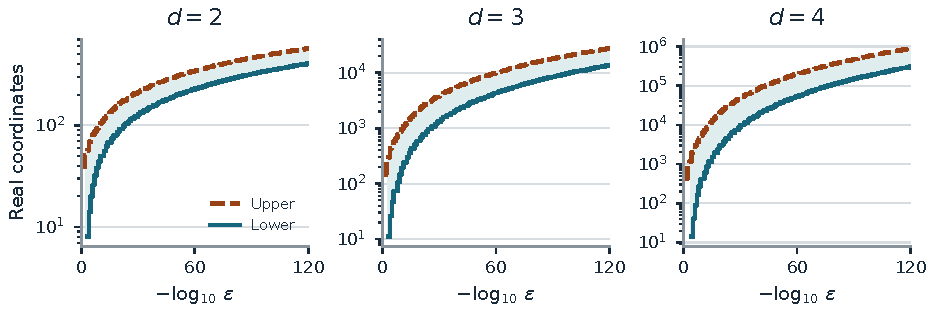
\includegraphics[width=.92\linewidth]{figures/dimension.pdf}
\caption{Finite, certified intervals for continuous state dimension at $p=2$ and $\beta=1$. The constructive and obstruction degrees are computed independently. Horizontal coordinates give the requested number of decimal digits of accuracy.}\label{fig:bounds}
\end{figure}

\section{Observable errors of an exact-key cache}
\label{app:math}
We give two different characterizations. The first asks how large the projected error can be when each value error lies in a prescribed interval. The second fixes the errors and asks whether \emph{any} query can detect them. Their quantifiers differ. Only the uniform corollary of the first is used by the codec.

\subsection{Shared values and the support function of a box}
Fix finite index sets for output coordinates $j$, query heads $h$, visible source positions $i$, value channels $c$, and groups $g$. For every head let $p_{hi}\ge0$ and $\sum_i p_{hi}=1$; masked positions can be assigned weight zero. Let $g(h)$ be its group. With real projection $W$ and fixed gates $s_{hc}$ define the linear map on shared residuals
\begin{equation}
 (Le)_j=\sum_{h,c}W_{j,hc}s_{hc}\sum_i p_{hi}e_{g(h),i,c}.
 \label{eq:L}
\end{equation}
It models the exact-arithmetic difference when values alone change. The two evaluations must share the same keys, queries, mask and gates.

\begin{theorem}[Sharp radius for shared value errors]\label{thm:box}
Let $0\le\eta_{gic}<\infty$. Set $a_{j,gic}=\sum_{h:g(h)=g}W_{j,hc}s_{hc}p_{hi}$. Then
\begin{equation}
 \max_{|e_{gic}|\le\eta_{gic}}\normi{Le}
 =\max_j\sum_{g,i,c}\eta_{gic}|a_{j,gic}|.
 \label{eq:box}
\end{equation}
For $|s_{hc}|\le1$ and $\eta_{gic}\le\eta$, this radius is at most $\eta\opnorm{W}$, with $\opnorm{W}=\max_j\sum_{h,c}|W_{j,hc}|$.
\end{theorem}
\begin{proof}
Collect the coefficients of each independently bounded shared residual in \eqref{eq:L}. The triangle inequality gives the right-hand side of \eqref{eq:box} as an upper bound. For a maximizing row $j_\star$, set $e_{gic}=\eta_{gic}\operatorname{sign}(a_{j_\star,gic})$, taking zero where the coefficient vanishes. The $j_\star$ coordinate attains the bound. Applying the triangle inequality inside each $a_{j,gic}$ and summing $p_{hi}$ over $i$ proves the uniform estimate.
\end{proof}

\paragraph{A strict cancellation.}
Two heads read the same scalar value residual at the same distribution, with gates one and output weights $+1,-1$. The exact radius is zero for every box. Giving each head an independent residual would produce a radius $2\eta$ for uniform tolerances. Conversely, for one head with gate one, all residuals can have the sign of the corresponding projection coefficient, so the universal constant in the uniform estimate cannot be reduced.

\paragraph{Instantiating the budget.}
If $W\ne0$, choose $\eta\le1/(128\opnorm W)$. Both the row encoder and raw fallback enforce $|e_{gic}|\le\eta$; raw rows give zero codec error. The resulting bound applies after the ideal linear output projection and before any subsequent rounding. For $W=0$ the projected error is identically zero. For a floating-point execution one can write
\begin{equation}
 \normi{\widehat y_{\rm compact}-\widehat y_{\rm dense}}
 \le \rho_{\rm compact}+\normi{Le}+\rho_{\rm dense},
 \label{eq:round}
\end{equation}
where each $\rho$ bounds that backend's deviation from its own ideal arithmetic at the specified inputs. No $\rho$ was measured here. The packed reader, for example, casts its tile probabilities to BF16 for the value product. A shared token history alone does not make the two networks' hidden states, keys or gates equal.

\subsection{Which residuals are invisible to every query?}
For a stronger identifiability question we impose more structure. Let an open set $U\subset\R^d$ of query parameters be nonempty, $d\ge1$. For each head $h=1,\ldots,H$ take a nonempty finite visible set $I_h$, effective keys $k_{hi}\in\R^d$, positive base weights $b_{hi}$, and fixed projected residual vectors $r_{hi}\in\R^m$. For grouped reads one may take $r_{hi}=W_h D_h e_{g(h),i}$ with a fixed diagonal gate $D_h$. The head scores are affine in the common parameter $x$; different linear query maps can be absorbed into the effective keys. The mask is fixed throughout $U$ and the gates are frozen. Define
\begin{align}
 Z_h(x)&=\sum_{i\in I_h} b_{hi}e^{\langle x,k_{hi}\rangle},&
 D(x)&=\sum_{h=1}^H
   \frac{\sum_{i\in I_h} b_{hi}r_{hi}e^{\langle x,k_{hi}\rangle}}{Z_h(x)} .
 \label{eq:visible}
\end{align}
Here $D(x)$ is the projected multihead perturbation. It is an analytic function in this restricted family.

\begin{theorem}[Exact observable quotient]\label{thm:quotient}
For $u=(i_1,\ldots,i_H)\in\prod_h I_h$, put $s(u)=\sum_h k_{h i_h}$, $b(u)=\prod_h b_{h i_h}$ and $r(u)=\sum_h r_{h i_h}$. Let $S=\{s(u)\}$ contain the distinct key sums and set
\begin{equation}
 C_s=\sum_{u:\,s(u)=s} b(u)r(u).
 \label{eq:classes}
\end{equation}
Then $D$ vanishes throughout $U$ if and only if $C_s=0$ for every $s\in S$. Two residual arrays induce identical functions on $U$ precisely when their difference lies in the kernel of the linear map $r\mapsto(C_s)_{s\in S}$. In particular its image is a concrete realization of the quotient by invisible residuals.
\end{theorem}
\begin{proof}
All $Z_h$ are positive. Multiply \eqref{eq:visible} by their product and expand. In the contribution of head $h$, the numerator supplies one $r_{h i_h}$, while all other heads supply just their denominator factors. Collecting identical exponent vectors gives
\begin{equation}
 D(x)\prod_h Z_h(x)=\sum_{s\in S} C_s e^{\langle x,s\rangle}.
 \label{eq:exp}
\end{equation}
Zero coefficients therefore suffice. Conversely choose $v$ outside the finite union of hyperplanes $\langle v,s-s'\rangle=0$ for $s\ne s'$. Fix $x_0\in U$ and choose a sufficiently small $\tau>0$ so all $x_j=x_0+j\tau v$, $0\le j<M=|S|$, lie in $U$. At these points the right side is a Vandermonde system in $z_s=e^{\tau\langle v,s\rangle}$, with vector coefficients $C_s e^{\langle x_0,s\rangle}$. The $z_s$ are distinct, so the system is invertible coordinatewise. Vanishing at the selected points forces all $C_s=0$. The last assertion follows from linearity and the first isomorphism theorem.
\end{proof}

\begin{corollary}[Finite witnesses and a stability bound]\label{cor:probe}
With the probes above and $V_{js}=z_s^j$, write $Z(x)=\prod_h Z_h(x)$. For exact real arithmetic,
\begin{equation}
 \max_s e^{\langle x_0,s\rangle}\normi{C_s}
 \le \opnorm{V^{-1}}\;\max_{0\le j<M}Z(x_j)\normi{D(x_j)} .
 \label{eq:conditioning}
\end{equation}
If a coefficient is nonzero, at least one of these $M$ probes detects the residual.
\end{corollary}
\begin{proof}
Stack \eqref{eq:exp} at the chosen probes and apply $V^{-1}$ to each output coordinate. Taking absolute row sums gives \eqref{eq:conditioning}.
\end{proof}

For a single head, \eqref{eq:classes} groups equal keys and takes a weighted sum of their projected residuals. At distinct keys all such residual vectors must individually vanish; duplicate keys can conceal cancellation. With several heads a coordinate's residual can instead cancel across heads. The number $M$ can be as large as $\prod_h |I_h|$. This is an identifiability result and may be prohibitively expensive as an algorithm. No claim is made that model-generated queries range over $U$ with fixed gates.

\paragraph{Why identification can be arbitrarily unstable.}
Take one scalar head, two distinct scalar keys $0,\delta$ with $\delta>0$, unit base weights and scalar projected residuals $+1,-1$. On $[-R,R]$ with $R>0$,
\begin{equation}
 D(x)=\frac{1-e^{\delta x}}{1+e^{\delta x}}=-\tanh(\delta x/2),
 \qquad \sup_{|x|\le R}|D(x)|=\tanh(R\delta/2).
 \label{eq:near}
\end{equation}
Both residual magnitudes are one. As $\delta\downarrow0$ the observation uniformly approaches zero despite exact identifiability for every $\delta>0$. Thus the inverse problem admits no separation-independent Lipschitz constant on that bounded query set. At $\delta=0$ the residual is exactly invisible.

\begin{corollary}[Affine sigmoid gates]\label{cor:gates}
The finite coefficient test extends to a finite collection of channel gates
$s_a(x)=u_a(x)/(1+u_a(x))$, where $u_a(x)=\gamma_a e^{\langle x,\lambda_a\rangle}$ and $\gamma_a>0$. Suppose each contribution to a projected coordinate is a fixed linear coefficient times an attention probability from \eqref{eq:visible}, a value residual, and one such gate. Multiply its total error by
\begin{equation}
  \left(\prod_h Z_h(x)\right)\left(\prod_a[1+u_a(x)]\right).
\end{equation}
Expand the product and collect equal exponent vectors. The coordinate error vanishes on any nonempty open $U$ if and only if each grouped scalar coefficient vanishes.
\end{corollary}
\begin{proof}
Every denominator is strictly positive. After cancellation, each summand is a product of constants, exponentials and factors $1+u_a$ from the other gates. Distributing the factors gives a finite exponential sum. Independence on an open set follows from the same finite Vandermonde argument as in Theorem~\ref{thm:quotient}. This proof permits negative projections and coincident exponent vectors.
\end{proof}
For example, the cancellation $\sigma(x)+\sigma(-x)-1=0$ is visible after writing $z=e^x$ and clearing the common denominator $1+z$. More generally, the coefficient test applies to affine-score, affine-gate families; input-dependent query normalization in a full model need not have this form.


\subsection{What changes when the mask moves?}
\begin{proposition}[Causal-prefix identification]\label{prop:causal}
Consider one head, a fixed linear projection and gate, and projected residuals $r_1,\ldots,r_n$ shared across all prefix experiments. At prefix $t$ observe $d_t=\sum_{i\le t}p_{ti}r_i$, with known weights and $p_{tt}>0$. Then $d_1=\cdots=d_n=0$ if and only if all $r_i=0$. More generally,
\begin{equation}
 r_t=(d_t-\sum_{i<t}p_{ti}r_i)/p_{tt}. \label{eq:causal}
\end{equation}
\end{proposition}
\begin{proof}
The observation matrix is triangular with diagonal $p_{tt}$. Forward substitution gives \eqref{eq:causal} and proves injectivity. A small diagonal can amplify perturbations, including earlier inversion errors.
\end{proof}
Thus even duplicate keys can be separated by a sequence of prefix observations under a common projection. The six recorded generations supply token IDs and selected logit summaries; they do not provide these prefix-wise projected measurements.

\subsection{From a local error to a token decision}
Let $x_t$ be a complete dense decoder state, including its cache, and $\tilde x_t$ its approximate counterpart. Until the first divergent greedy token, both receive the same discrete input $u_t$. Suppose the exact state update $F_t(\cdot,u_t)$ is $L_t$-Lipschitz on a region containing both trajectories, and the approximate update differs from it by at most $\epsilon_t$ on that region, in a specified state norm. If the dense logit readout is $M_t$-Lipschitz into $\ell_\infty$ and its approximate counterpart has error at most $\xi_t$, then with $\delta_0=\norm{x_0-\tilde x_0}$ (in the chosen norm),
\begin{align}
 \delta_t &\le
 \delta_0\prod_{k=0}^{t-1}L_k+
 \sum_{j=0}^{t-1}\epsilon_j\prod_{k=j+1}^{t-1}L_k,
 &\|\tilde z_t-z_t\|_\infty&\le M_t\delta_t+\xi_t. \label{eq:state}
\end{align}
Here $\norm{x}$ denotes the chosen state norm and an empty product is one. The first inequality follows by iterating $\delta_{t+1}\le L_t\delta_t+\epsilon_t$, the second by inserting the exact readout at $\tilde x_t$. If the dense top-two logit margin at time $t$ strictly exceeds $2(M_t\delta_t+\xi_t)$, its maximizing token is unchanged: each competitor can close the gap by at most twice the logit error. Applying this test inductively certifies a finite greedy path when all hypotheses hold at every step. No such state constants or margins were logged for the run. Its token agreement is an observation.

\paragraph{Executable witnesses.}
The companion's \texttt{tools/math\_checks.py} enumerates all 16 corners of a shared two-head residual box using rational arithmetic; directly evaluates a cancelling two-head example; verifies the cleared numerator at finite probes with collisions; and checks a duplicate-key cancellation. These small cases test the indexing and order of summation. The general results follow from the proofs above.

\section{The one-reference problem}\label{app:one}
Fix integers $b\ge1$ and $g\ge1$, a finite integer domain $D=\{0,\ldots,2^b-1\}$ and nonempty groups of magnitudes in $D$. The domain is discrete throughout. Write $B=b+1$. All proofs concern encoded bit patterns. A NaN is a legal word.

Let a magnitude occupy $b$ bits. For binary32, $b=31$ and $a_i=u_i\bmod 2^{31}$, where $u_i$ is the stored unsigned word. The sign bit travels separately. Exponents and fraction fields remain part of $a_i$, including for signed zeros, infinities and NaN payloads. For a stored reference $p\in D=\{0,\ldots,2^b-1\}$ define
\[
 \zz(d)=\begin{cases}2d&d\ge0,\\-2d-1&d<0,\end{cases}
 \qquad w_j(p)=\bitlen\!\left(\max_{i\in G_j}\zz(a_i-p)\right).
\]
Here $\bitlen(0)=0$ and $\bitlen(x)=1+\lfloor\log_2 x\rfloor$ otherwise. Each of the $g$ groups $G_j$ is nonempty. Its minimum and maximum are $l_j,h_j$. The largest possible width is $B=b+1$.

\begin{theorem}[Exact reference selection]\label{th:sweep}
Let $f_j(w)$ be any nondecreasing group cost on $\{0,\dots,B\}$, including byte rounding. For $1\le t<B$ let
\[
 I_{jt}=D\cap[h_j-2^{t-1}+1,\ l_j+2^{t-1}].
\]
At $t=0$ use the singleton $\{l_j\}$ when $l_j=h_j$, and the empty set otherwise. Give $I_{jt}$ weight $f_j(t+1)-f_j(t)$. If $M$ is the maximum total weight of intervals containing one point of $D$, then
\[
 \min_{p\in D}\sum_{j=1}^{g} f_j(w_j(p))=\sum_{j=1}^{g} f_j(B)-M.
\]
A sweep of the interval endpoints returns an attaining reference in $O(gB\log(gB))$ time and $O(gB)$ space after reading the group extrema.
\end{theorem}

The asymmetric $+1$ at the left endpoint matters. For a one-bit group the two encodable differences are $-1$ and $0$. The condition $w_j(p)\le t$ is exactly $p\in I_{jt}$. Summing the weights of the satisfied thresholds telescopes from $f_j(B)$ down to the actual cost. Sorting starts and one-past-ends turns this identity into an algorithm. The supplement proves the endpoint convention, the certificate and the extension to a shared codebook of $k$ references.


The tested layout groups a row of 128 words into sixteen groups of eight. Denote by $s$ the number of nonempty 32-word sign-exception masks, relative to the first word's sign. The residual row length in bytes is
\[
 R(p)=17+4s+\sum_{j=1}^{16} w_j(p).
\]
One descriptor, four reference bytes and twelve width bytes account for the constant 17. The masks are lossless. The shortest alternative $A$ ranges over raw storage, rowwise exponent offsets, four local exponent ranges, and an all-positive-zero escape when admissible. The encoder selects $F(p)=\min\{A,R(p)\}$. A four-byte length and one nonempty-head tag frame all 128 rows. No empirical size table assumes free headers.

\begin{proposition}[Attainable savings and a format lower bound]\label{th:lower}
Write $R_*=\min_p R(p)$, and let $R_0$ be the residual length of any fixed policy. The improvement in the complete row is exactly
\[
 \min(A,R_0)-\min(A,R_*)=[\min(R_0-R_*,A-R_*)]_+ .
\]
Even if every group receives its own free reference, the shortest row with the existing residual header and alternative modes has length
\[
 L_{\rm free}=\min\left\{A,\;17+4s+\sum_j\bitlen(h_j-l_j)\right\}.
\]
It is a lower bound for every shared-reference or multiple-reference scheme using this layout and nonnegative additional overhead. If the residual term inside the braces is at least $A$, the encoder can skip the sweep and emit the winning alternative.
\end{proposition}


\subsection{Thresholds, costs and certificates}
\begin{lemma}[Feasible references for one threshold]\label{lem:threshold}
For $t\ge1$, the group permits width at most $t$ exactly on
$D\cap [h_j-2^{t-1}+1,\ l_j+2^{t-1}]$. Width zero is possible precisely when the group is constant and $p$ is that constant.
\end{lemma}
\begin{proof}
The image of $\zz$ on the consecutive integers from $-2^{t-1}$ through $2^{t-1}-1$ is exactly $\{0,\ldots,2^t-1\}$. Hence all residuals fit if and only if $a_i-2^{t-1}+1\le p\le a_i+2^{t-1}$ for every $i$. Intersect these bounds and $D$. For $t=0$, the only valid residual is zero. This argument includes $p=0$ and $p=2^b-1$.
\end{proof}
\begin{proof}[Proof of the exact reference-selection theorem]
Let $v_{jt}=f_j(t+1)-f_j(t)\ge0$. Since the threshold intervals are nested, a point $p$ belongs precisely to those with $w_j(p)\le t<B$. Thus
\[
 \sum_{t=0}^{B-1}v_{jt}\ind\{p\in I_{jt}\}
 =\sum_{t=w_j(p)}^{B-1}(f_j(t+1)-f_j(t))=f_j(B)-f_j(w_j(p)).
\]
Summing over $j$ proves the threshold identity. For each nonempty integer interval $[L,U]$, add $+v_{jt}$ at $L$ and $-v_{jt}$ at $U+1$. Include $0$ as a candidate of zero initial depth, aggregate coincident events before taking a maximum, and disregard the sentinel $2^b$ as a candidate. The prefix sum is constant up to the next event, so the greatest prefix sum is the maximum feasible depth. Sorting at most $2gB$ events gives the stated time and memory bounds under constant-time endpoint arithmetic. Directly computing frequencies or enumerating all $2^b$ references is unnecessary.
\end{proof}

\paragraph{Verifiable optimum.} A certificate consists of the extrema, a proposed $p$, and the sorted event coordinates with their aggregated signed weights. The verifier independently reconstructs the events, then checks every prefix sum and evaluates the actual width at $p$. Equality of $\sum_jf_j(w_j(p))$ with the constant minus the largest prefix proves optimality. When the sorted multiset is trusted, verification takes $O(gB)$ operations. Independent reconstruction and sorting take $O(gB\log(gB))$. Checking the length at the proposed reference alone would certify only feasibility.

\paragraph{A worked record.} In the five-group example, $g=5$ and $k=5$. At $p=40$ the common value has residual $-16$ with code 31. The outlier has residual $+16$ with code 32. The resulting widths are $(5,5,5,5,6)$. At $p=24$ they are $(0,0,0,0,7)$. Changing $p$ to 25 would give width one to all four constant groups, which already outweighs a one-bit saving in the fifth.


\begin{figure}[ht]
\centering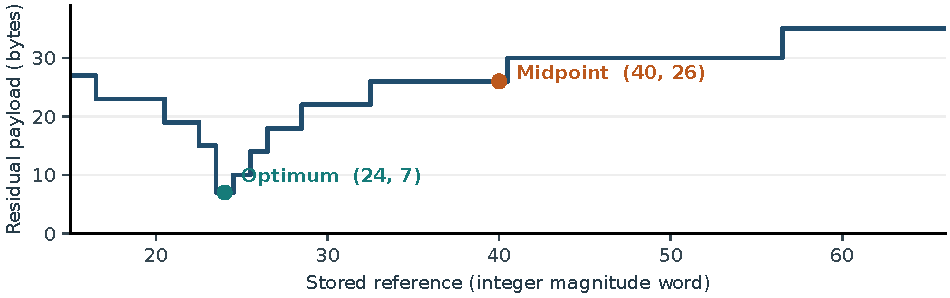
\includegraphics[width=.84\linewidth]{figures/reference_cost.pdf}
\caption{Exact cost of the five-group witness. Each width unit is one byte for a group of eight words.}\label{fig:exampleagain}
\end{figure}

\begin{proposition}[One-outlier separation]\label{th:gap}
For $g\ge2$ groups of eight, $k\ge1$, and $0\le m\le 2^b-1-2^k$, take one magnitude $m+2^k$ and all others $m$, with the outlier in a mixed group. The difference between the midpoint and minimum residual payload is $(g-1)k-1$ bytes.
\end{proposition}
\begin{proof}
At $p=m+2^{k-1}$ the constant groups need width $k$, and the mixed group needs $k+1$. At $p=m$ the common groups cost zero, while the outlier code is $2^{k+1}$ and costs $k+2$. For any other reference, each constant group costs at least one. A width $k$ covers at most $2^k$ consecutive magnitudes, while the mixed group spans $2^k+1$ possible integer positions from its minimum to its maximum inclusive. Hence it costs at least $k+1$ for every reference. Consequently every $p\ne m$ costs at least $(g-1)+(k+1)\ge k+2$. Subtract the two attained values. At $g=2,k=1$ the gap is zero, as the formula predicts.
\end{proof}

\section{Relaxations, screening and more than one reference}\label{app:multiple}
\begin{lemma}[Independent group optimum]\label{lem:span}
For $d=h-l$, $\min_{p\in D}w(p)=\bitlen(d)=\lceil\log_2(d+1)\rceil$.
\end{lemma}
\begin{proof}
For $d=0$ take $p=l$. For $d>0$ a width-$t$ signed code spans at most $2^t-1$ in magnitude difference, so $d\le2^t-1$ is necessary. For the least such $t$, $h-2^{t-1}+1\le l+2^{t-1}$. The left boundary is at most $h$ and the right boundary is at least $l$, so this interval intersects $D$. The threshold lemma supplies a feasible reference. This includes spans $2^t-1$ at equality.
\end{proof}
\begin{proof}[Proof of the complete-format bound]
For numbers $x\ge y$, $\min(A,x)-\min(A,y)$ equals zero for $A\le y$, equals $A-y$ for $y<A<x$, and equals $x-y$ for $A\ge x$. Apply this identity to $x=R_0,y=R_*$. Give each group an independent reference as free side information, keeping the header and sign-mask rules fixed. Group widths can now achieve their separate minima simultaneously, so the formula for $L_{\rm free}$ follows from Lemma~\ref{lem:span}. Choosing an existing alternative is still allowed. If the independent-reference residual length is at least $A$, every genuine residual scheme with this layout is at least as expensive as $A$. The encoder's fixed tie rule gives priority to the alternative, which then determines the same serialized record.
\end{proof}

\paragraph{An even cheaper hypothetical format.} Give the decoder all signs and all group references, including the first reference, for free. Charge only the one-byte descriptor, twelve width bytes and the group payloads. Its per-row floor is
\[
 \min\{A,\ 13+\textstyle\sum_j\bitlen(h_j-l_j)\}.
\]
This is an attainable length with that side information, and a lower bound when it must be transmitted. All nonempty heads retain the original five framing bytes. The aggregate is 142,111,471 bytes, exceeding the bit-shuffled control by just 17,574 bytes (0.0124\% of the control). This second gap is sensitive to framing and checkpoint mix. A different entropy code for the widths, variable group boundaries, or another alternative row mode would define a different family.

\subsection{The optimum with a shared codebook}
Let $P\subseteq D$ be a set of at most $k$ references, $k\ge1$. Each group may select a reference independently. Suppose that headers and reference-index costs are fixed once $k$ is chosen. A fixed selector of $\lceil\log_2 k\rceil$ bits per group satisfies this assumption. Variable costs depending on the selected index require another objective.
\begin{theorem}[Codebook reduction]\label{th:multiple}
For the costs in the one-reference theorem, minimizing
$\sum_j\min_{p\in P} f_j(w_j(p))$ is equivalent to maximizing the total interval weight hit by at least one point of $P$. Some optimum uses only $0$ and left endpoints of nonempty threshold intervals.
\end{theorem}
\begin{proof}
The interval family is nested for each group, and $f_j$ is nondecreasing. The thresholds hit by any point in $P$ are exactly the thresholds at or above $\min_{p\in P}w_j(p)$. Telescope the cost as before. For the second statement, remove any point that hits nothing. For each remaining point replace it with the largest left endpoint of the intervals that it hits. That value is no larger than the point and still lies in every previously hit interval. Coincident replacements can be merged. With zero total weight the point $0$ is sufficient.
\end{proof}

\paragraph{Dynamic program and certificate.} Sort the $m$ distinct candidate coordinates as $x_1<\cdots<x_m$. Use a sentinel $x_0=-1$. For $i<j$ let
\[
 H(i,j)=\sum_{[L,U]}v_{LU}\ind\{x_i<L\le x_j\le U\}.
\]
If the previous rightmost selected point is $x_i$, an interval containing $x_j$ is new precisely when $L>x_i$. Indeed, if $L\le x_i$ it already contains $x_i$, while if $L>x_i$ every earlier point is too far left. With $D_1(j)=H(0,j)$, the recurrence
\[
 D_r(j)=\max_{i<j}\{D_{r-1}(i)+H(i,j)\}
\]
therefore computes the best covered weight with $r$ ordered points ending at $x_j$. Unreachable states are $-\infty$. Take the maximum over $r\le\min(k,m)$ and $j$, allowing the empty solution of value zero. Backpointers give attaining references. For $n$ nonempty threshold intervals one may tabulate $H$ in $O(m(n+m))$ time: for each right candidate bin the active interval weights by their left endpoints and take suffix sums. The dynamic program then costs $O(km^2)$ time, with $O(m^2+km)$ space including reconstruction. Classical partial interval hitting admits other algorithms \cite{hitting}. Our use is an exact benchmark for this byte cost. The multi-reference formula has been checked on finite examples. The corpus measurements executed the single-reference encoder.

\section{Word identity and the limits of geometric evidence}\label{app:words}
\begin{proposition}[Lossless transport through a deterministic update]\label{th:transport}
Let $E,D$ encode and decode a state of machine words with $D(E(x))=x$ on all reachable states. Consider a deterministic native transition and output $(x',y)=T(x,u)$ whose other state, arithmetic environment and input sequence are identical in both runs. The wrapped transition forms $(x',y)=T(D(c),u)$ and stores $E(x')$. Starting from $c_0=E(x_0)$ yields equal native state and output words at every step.
\end{proposition}
\begin{proof}
Initially the decoded state agrees by assumption. At any step equal input and resident auxiliary state give identical arguments to $T$ and hence identical output and next native state. Applying $D\circ E$ preserves that state for the next step. This induction also covers a sampler if its state and random draws agree. Integer residual storage satisfies the premise because $p+\zz^{-1}(\zz(a-p))=a$ and XOR with a saved sign mask is its own inverse. The exponent modes invert integer offsets and copy every other field. Raw storage and the positive-zero escape have explicit inverses. Bytewise equality avoids the ambiguity of floating-point comparisons at signed zero or NaNs.
\end{proof}
Changing reduction order, floating-point contraction, sampler state or the native transition changes the hypotheses. The storage replay in this paper checks the codec premise on the archived words. It does not execute a new online model transition.

\begin{theorem}[A high-energy rank-one component can hide arbitrary bits]\label{th:rank}
For positive integers $m,n$ and $1\le s\le23$, there are $2^{smn}$ distinct positive binary32 matrices $X$ for which the rank-one matrix $J=\mathbf1\mathbf1^\top$ satisfies
\[
 \frac{\lVert X-J\rVert_F^2}{\lVert X\rVert_F^2}
 \le ((2^s-1)2^{-23})^2 .
\]
Every injective binary representation has worst-case length at least $smn$ bits on this family. A prefix-free representation has uniform expected length at least $smn$ bits.
\end{theorem}
\begin{proof}
Independently choose $d_{ij}\in\{0,\ldots,2^s-1\}$ and set $X_{ij}=1+2^{-23}d_{ij}$. Binary32 represents all of these numbers exactly within the same exponent bin. The numerator is at most $mn((2^s-1)2^{-23})^2$ and the denominator is at least $mn$. Fewer than $2^{smn}$ binary strings have length strictly below $smn$, which proves the worst-case bound. For a prefix code of lengths $L_i$, Kraft's inequality and convexity give $2^{-\mathbb E L}\le \mathbb E2^{-L}\le2^{-smn}$ under the uniform law.
\end{proof}
For $s=12$, the relative squared error is below $2.39\times10^{-7}$ while 12 freely chosen bits per entry remain. This construction is a counting obstruction to using an approximation score as a lossless code-length guarantee. Structured states outside the family can compress much further.

\section{Records, protocols and checks}\label{app:experiment}
\subsection{Exactly what is on the wire}
A layer dump stores sixteen little-endian FP32 heads. Within a head, the row decoder reads 128 consecutive self-delimiting records. For a nonzero head, the four-byte unsigned payload length precedes a one-byte head tag and the records. An all-positive-zero head uses a zero length and no head tag or row bytes. The dense baseline costs exactly 65,536 bytes per head. The code checks the machine byte order before replay.

\begin{center}\small
\begin{tabular}{ll}\toprule
Row mode & Serialized bytes per 128-word row \\ \midrule
Raw & $1+512$ \\
One exponent minimum and width $e$ & $386+16e$ \\
Four local minima and widths $e_t$ & $391+4\sum_{t=1}^4e_t$ \\
Integer magnitude residual & $17+4s+\sum_{j=1}^{16}w_j$ \\
All positive zeros & $1$ \\ \bottomrule
\end{tabular}
\end{center}
Exponent offsets take the unsigned bit length of the exponent span. The sign and 23 fraction bits occupy three bytes per word. In the residual mode the reference word holds a 31-bit reference magnitude and the sign of the first word. Each 32-word tile stores a four-byte XOR sign mask only when some sign differs from the reference sign. Six bits per group width suffice for values 0 through 32, even when residuals reach 32 bits. Bit packing is least-significant bit first. The baseline midpoint is the floor of $(\min a+\max a)/2$ evaluated in widened integer arithmetic. The lower median is order statistic 64 among 128 values. On ties the nonzero encoder chooses raw, then row exponents, then local exponents, then residuals. This tie convention also allows the screened encoder to reproduce the unscreened stream byte for byte. Row records are sequentially parseable. A random-row offset table would incur additional bytes.

The whole-head controls use the same granularity and wrapper accounting as each other. A tag identifies the transformation and compressor, and a four-byte unsigned length delimits the frame. The byte shuffle concatenates the four byte lanes of the entire head. The bit shuffle transposes contiguous blocks of 256 words into 32 bit planes. A single Zstandard frame covers the transformed head. Each baseline falls back to the native payload if compression fails to shorten it. Sizes describe these explicitly implemented serializations. No indexes across heads, allocator capacity, Python objects or resident model weights are included.

\subsection{Results by checkpoint and recurrent layer}
\begin{table}[ht]\centering\small
\caption{Saving from replacing the midpoint with the exact reference. Each checkpoint comprises 864 heads and 110,592 rows. Retained is the complete-format gain divided by the residual-only gain.}\label{tab:checkpoints}
\begin{tabular}{rrrrr}\toprule Token & Residual bytes saved & Frame bytes saved & Retained & Rows shortened \\ \midrule
\tabinput figures/checkpoints.tex 
\bottomrule\end{tabular}
\end{table}
\begin{figure}[ht]\centering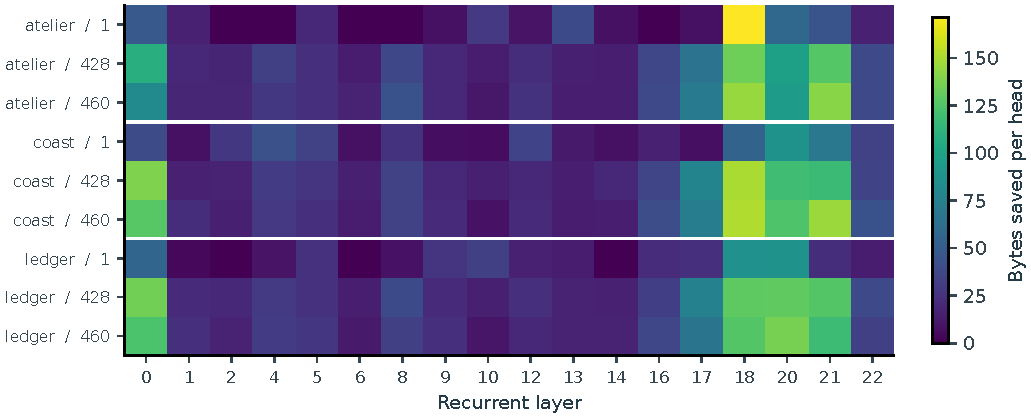
\includegraphics[width=\linewidth]{figures/layers.pdf}
\caption{Complete-format savings from exact reference selection. Each cell is the mean difference in bytes over the 16 heads of the indicated layer, trace and token. All 18 recurrent layers are included. Early checkpoint measurements differ visibly by layer.}\label{fig:layer}
\end{figure}
\begin{table}[ht]\centering\small
\caption{Dependence on the saved token. The last two columns compare head frames. Free sides is the lower bound with all group references and signs supplied for free.}\label{tab:free}
\begin{tabular}{rrrrr}\toprule Token & Fixed-header floor & Free sides & Optimal local & Bit shuffle + Zstd \\ \midrule
\tabinput figures/floors.tex 
\bottomrule\end{tabular}
\end{table}
The residual mode wins 3,858 rows at the midpoint and 39,694 under optimal selection. A rise in the number of wins can accompany a small change in bytes because a new residual winner must first cross the competing exponent record. Table~\ref{tab:checkpoints} quantifies this effect. The 17,574-byte gap in the more permissive relaxation is an aggregate across the three equally weighted positions. Table~\ref{tab:free} shows why this number cannot be extrapolated to a steady-state distribution of token ages.

\begin{figure}[ht]\centering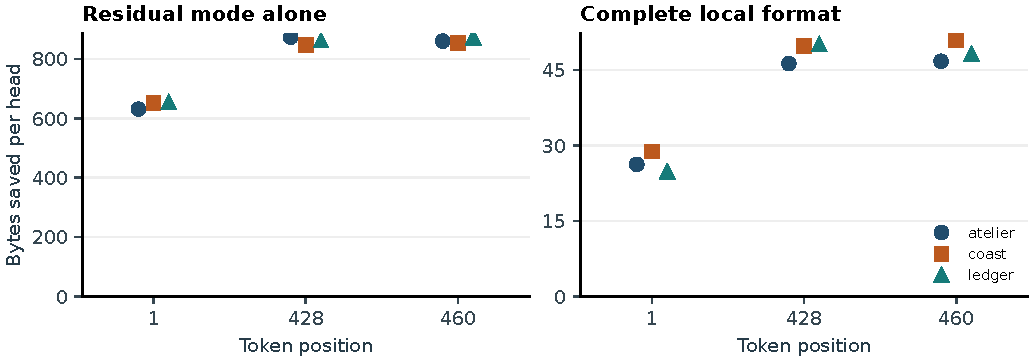
\includegraphics[width=.94\linewidth]{figures/mode_competition.pdf}
\caption{Savings from the optimal reference before and after mode selection. Each point averages 288 heads at one trace and checkpoint. Each panel has its own byte scale.}
\end{figure}
\begin{table}[ht]\centering\small
\caption{All measured lossless controls. Sizes include head framing for each coded representation.}
\begin{tabular}{lrrr}\toprule Method & Bytes & Bits per word & Saved (\%)\\\midrule
\tabinput figures/sizes.tex
\bottomrule\end{tabular}
\end{table}
\subsection{An adaptive head frame}\label{app:mixed}
For head $i$, let $a_i$ and $b_i$ be the complete serialized local-optimal and bit-shuffle/Zstandard lengths. We concatenate one unsigned selector byte followed by the chosen intact frame. Selector zero indicates the local format; selector one indicates bit shuffle, including its own raw fallback. Both inner formats already delimit their payload with a four-byte little-endian length, so a decoder can walk the concatenation with no external offsets. Ties select bit shuffle. For $H$ heads the allocation is exactly $H+\sum_i\min(a_i,b_i)$. Against always storing the bit-shuffled frame, the net gain is $\sum_i[b_i-a_i]_+-H$. With this wrapper, local optimality of choosing the shorter frame follows from separability over heads.

\begin{table}[ht]\centering\small
\caption{Fresh serialization and bytewise readback of the two-format stream. Each token position contributes 864 heads. All byte totals include the one-byte outer selector per head.}
\begin{tabular}{rrrr}\toprule Token position & Local selected & Shuffle selected & Mixed bytes\\\midrule
1 & 0 & 864 & 42,040,298\\
428 & 777 & 87 & 49,384,814\\
460 & 745 & 119 & 49,310,794\\\midrule
All & 1,522 & 1,070 & 140,735,906\\\bottomrule\end{tabular}
\end{table}
We ran the original four-policy replay and the mixed encoder on all 42,467,328 native FP32 words. For each head the census replay matched the stored counts and the mixed decoder matched the raw input and the recorded SHA-256. The mixed encoder constructs both candidates in memory. The extra encoding latency, peak transient memory and online access pattern are open performance questions.

\subsection{CPU microbenchmark and historical inference context}
\begin{table}[ht]\centering\small
\caption{In-memory encode-only timings for the bundled 162-head subset (10,616,832 input bytes per pass). Range is the minimum and maximum across eight post-warm-up passes. MB/s uses decimal input megabytes and median pass time.}\label{tab:time}
\begin{tabular}{lrrr}\toprule Reference policy & Median (ms) & Range (ms) & MB/s \\ \midrule
\tabinput figures/timings.tex 
\bottomrule\end{tabular}
\end{table}
One head per (trace, token, layer) was retained in the portable subset. Use zero-based layer ordinal $j$ in the sorted recurrent-layer list and trace ordinal $i$ in (atelier, coast, ledger). The retained head index is $(j+5i)\bmod16$. Selection is independent of the values and identical across token positions for each trace and layer. Every method encoded the same 162 heads. The timed C++ process was pinned to one logical CPU on an AMD EPYC 9V74 and built with GCC 14.2, \texttt{-O3 -std=c++17}. One unrecorded warm-up pass per policy preceded eight timed passes per policy. Starting order rotated across repeats. Input was already resident. The timed loop encoded into a preallocated buffer, including framing. A checksum consumed all output bytes outside the timer. Typical full verification also requires space for the 162 MiB original corpus, compiler output and per-row CSVs. No GPU or inference engine is needed to reproduce the codec results.

A separate historical integration \cite{archive} measured the \emph{midpoint} local format in Qwen3.5-0.8B-Q4\_K\_M, using four pinned CPU cores. Peak recurrent-matrix allocation was 18,874,368 bytes natively and 16,760,064 bytes in a locally fused implementation. Process peak RSS was 837,459,968 and 832,233,472 bytes respectively. A separate three-repeat timing protocol reported medians of 13.732 and 20.386 seconds. This historical result supports the decision to measure bytes and runtime separately. The current Q4\_0 snapshot study uses a different quantization and traces, and its new optimizer was run offline.

\subsection{Reproduction and numerical checks}
The companion notebook includes the complete per-head census, raw words for the 162-head portable replay, the C++ codec, an independent integer verifier and all plot sources. Its default CPU run regenerates the tables and figures from per-head observations and verifies the portable subset against those observations. The optional full-data input contains the original words for all 2,592 heads. Supplying it to the notebook repeats the entire census. The archived capture names are \texttt{Qwen\_GDN\_Full\_State\_Lossless\_Evidence.zip} and \texttt{Qwen\_GDN\_Full\_State\_Lossless\_Results.zip}. Sorted census order is trace, token, layer and head. For exact baseline sizes the reference environment used python-zstandard 0.25.0 with libzstd 1.5.7. The companion records zlib and other runtime versions. The portable replay compares the pinned local codec independently of external compressor versions.

\begin{itemize}\setlength\itemsep{1pt}
\item The Python verifier enumerates all 4,096 ordered four-symbol records over an eight-symbol alphabet with two groups, checking both one and two references by exhaustive codebook search. It also checks 180 fixed-seed four-group records each with one, two and three references, 116 outlier identities, and extreme 31-bit endpoints.
\item An independent C++ loop enumerates the same 4,096 records expanded to sixteen groups and compares the production endpoint sweep against direct reference enumeration. Across 128 constructed rows, 512 round trips exercise all five row modes and include both signs of zero, denormals, infinities and NaN payloads.
\item The census runner verifies every selected row length, per-row dominance, the complete-format identity and the independent-span floor. It decodes every serialized head and checks it against the raw bytes. The four general-purpose controls have separate inverse transformations.
\end{itemize}

The corpus consists of model-state words. It includes no model weights or user conversation transcripts. The Qwen base model card identifies its Apache 2.0 license \cite{qwen}. Shorter exact checkpoints can lower storage requirements, while the ability to reconstruct all state bits means that ordinary access restrictions for the uncompressed state also apply to its encoded form. A language model assisted with the derivations, manuscript and implementation. The proofs specify the claims supported by finite computation and distinguish the historical engine evidence from the new results.

\newcommand{\TimingRows}{%
Emma & 4,096 & 0.314 & 0.16 & 1.327 & 1.12 & 2.44 \\
Moby-Dick & 4,096 & 0.246 & 0.16 & 0.460 & 1.05 & 1.50 \\
Emma & 32,768 & 2.084 & 0.69 & 4.657 & 2.89 & 7.54 \\
Moby-Dick & 32,768 & 2.077 & 0.69 & 3.783 & 2.88 & 6.66 \\
Emma & 131,072 & 9.184 & 2.45 & 15.937 & 10.00 & 25.93 \\
Moby-Dick & 131,072 & 9.203 & 2.46 & 14.931 & 10.01 & 24.94 \\
}


\section{GPU protocol and measured timings}
\label{app:record}
\paragraph{Runtime.}
The trace records PyTorch 2.14.1+cu130, CUDA 13.0, Triton 3.8.0, FlashInfer 0.7.5.post1 and Transformers 5.5.0. The model revision is \texttt{2fc06364715b967f1860aea9cf38778875588b17}. Full-attention layer indices are 3, 7, 11, 15, 19 and 23 (zero-based). For the recurrent layers the reported decode function is \texttt{torch\_recurrent\_gated\_delta\_rule}. The reader uses four warps, one pipeline stage, and a split attention calculation followed by a reduction. The two backends share a fused gate/output projection. Weights, recurrent state, workspaces, status flags and allocator overhead are outside the reported KV capacity. In particular the compact partial-output and softmax-statistic buffers consume additional device memory.

\paragraph{Timing and aggregation.}
Disclosure of the timing boundary matters for a sub-percent effect. The clock starts after cloning recurrent state and synchronizing the GPU. Each call to \texttt{item()} makes the selected ID available on the host. A final synchronization precedes the end timestamp. Each backend reuses its built decoder across runs; suffix slots are overwritten and only the valid prefix plus current suffix is visible. The alternating order starts with a different backend on the two books at each context length. A pair's plotted change is $100(t_{\rm dense}/t_{\rm compact}-1)$ because token counts match. Pooled rates weight elapsed time by summing tokens and seconds before taking their ratio. Error ranges in the paired plot show all four observed ratios; they are not confidence intervals. The 48 timed runs total 38.52 seconds of generation. This excludes data loading, build, prefill, warm-up, probes and compilation outside the timers. The complete project-wide GPU-hour total was not logged.

\begin{table}[ht]
\centering
\caption{Measured prefill and build times, with reconstructed single-request totals. Dense build is reported in milliseconds; all other time columns use seconds. Totals add common prefill, method-specific build and the mean of four warm runs of 64 tokens. They exclude unrelated setup and compilation outside these stages.}
\label{tab:stage}
\begin{tabular}{lrrrrrr}\toprule
Book & Prefix & Prefill & Dense build & Compact build & Dense total & Compact total\\
 & (tokens) & (s) & (ms) & (s) & (s) & (s)\\\midrule
\TimingRows
\bottomrule\end{tabular}
\end{table}

\begin{figure}[ht]\centering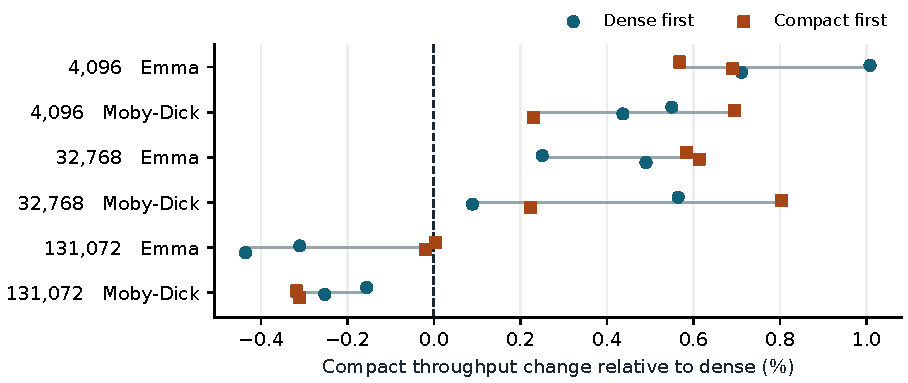
\includegraphics[width=.93\linewidth]{figures/paired.pdf}
\caption{The 24 within-condition timing pairs. The line spans the observed range, and the symbols give the order of the dense and compact runs. Positive change favors compact storage.}\label{fig:pairs}
\end{figure}
\paragraph{Where fallback occurs.}
Figure~\ref{fig:fallback} counts 768 appended rows per tensor and layer: two groups, 64 new positions and six conditions. Each condition contributes once. The value fallback changes from $0/768$ at layer 7 to $764/768$ at layer 23. These counts explain variation in logical suffix size. Reserved suffix capacity is independent of the fallback count. For the six layers in order, the recorded maximum absolute row sums of $W$ are 61.05, 36.40, 40.34, 38.46, 49.36 and 40.61 (rounded). In particular the final layer does not have the strictest nominal coordinate tolerance. These records alone cannot distinguish the effects of the realized exponent ranges and rounding residuals on each row.

\begin{figure}[ht]
\centering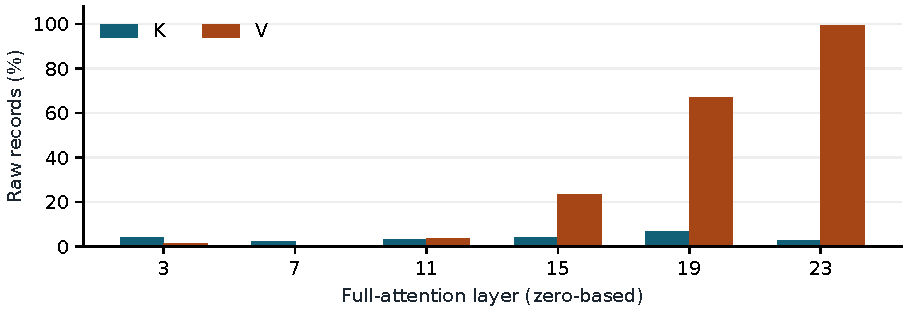
\includegraphics[width=.90\linewidth]{figures/fallback.pdf}
\caption{Fraction of appended records that use the full BF16 payload. Counts pool the six distinct prompt-length conditions, without counting timing repetitions. K and V use different fallback criteria.}
\label{fig:fallback}
\end{figure}

\paragraph{Independent arithmetic and integration checks.}
On a short prefix of 255 tokens, a separate probe compares each custom decode path with the original Hugging Face text decoder over four common-history steps, crossing the 256-position boundary. All eight backend--reference top choices agree. This checks integration at four positions only; the long-context dense baseline is the FlashInfer path described in the main text. The supplied CPU reference additionally exercises exact key round trips and four value budgets on 244 synthetic BF16 rows, including signed zeros, subnormals and wide exponent spreads. The corresponding script records the seed and tests raw as well as packed values. The long-context logits and continuations reported above come solely from the archived GPU trace.

\paragraph{Reproducing the paper.}
The artifact contains the measured JSON, model revision, corpus and token hashes, per-token times, generated IDs, verification scripts and GPU kernels. The CPU replay re-derives the tables, the three vector figures and the allocation identities. The optional fresh run uses a compatible NVIDIA stack, fetches the two source books and verifies their hashes. A new run writes to a separate location so the published measurements retain their identity. One source archive compiles with pdfLaTeX and includes the figures as PDFs. The notebook embeds the experiment scripts, CPU replay inputs and plotting code.

\paragraph{Scope, assets and disclosure.}
Qwen supplies the checkpoint under Apache-2.0. NLTK lists its Project Gutenberg selections as public domain; the companion retrieves upstream texts by hash and distributes neither books nor model weights. The benchmark concerns infrastructure for inference. Reducing cache storage could lower the cost of some deployments; increased capacity can also increase total use. The measurements contain no energy or emissions data. No human participants or personal evaluation records are involved. Generative AI assisted in drafting the analysis, deriving the mathematical presentation, writing verification and packaging code, and preparing the manuscript. The measurement claims are tied to the supplied run record.


\ifdefined\SupplementCopy\clearpage\begin{thebibliography}{99}
\bibitem{kath} A. Katharopoulos, A. Vyas, N. Pappas and F. Fleuret.
Transformers are RNNs: Fast autoregressive transformers with linear attention. \emph{ICML}, PMLR 119, 5156--5165, 2020.
\bibitem{schlag} I. Schlag, K. Irie and J. Schmidhuber.
Linear transformers are secretly fast weight programmers. \emph{ICML}, PMLR 139, 9355--9366, 2021.
\bibitem{haris} T. Haris and K. Onak.
Compression barriers in autoregressive transformers. \emph{COLT}, PMLR 291, 2757--2785, 2025.
\bibitem{balance} E. Kochetkova, K. J. Sheth, I. Han, A. Zandieh and M. Kapralov.
Streaming attention approximation via discrepancy theory. \emph{Advances in Neural Information Processing Systems} 38, 2025.
\bibitem{chen} J. Y. Chen, Y. Feng, P. Indyk, M. Kapralov, E. Kochetkova and B. Prokhorov.
Towards tight bounds for streaming attention. \href{https://arxiv.org/abs/2606.07205}{arXiv:2606.07205}, 2026.
\bibitem{risk} L. Haverbeck, C. Amo Alonso, A. F. Posada-Moreno, S. Trimpe and M. Pavone.
The risk of KV cache compression. \href{https://arxiv.org/abs/2607.01520}{arXiv:2607.01520v2}, 2026.
\bibitem{entropy} K. Gonzalez and T. Jord\~ao. A close look at the entropy numbers of the unit ball of the reproducing Hilbert space of isotropic positive definite kernels. \emph{Journal of Mathematical Analysis and Applications}, 534(2), 2024. \url{https://arxiv.org/abs/2304.14103}.
\bibitem{devore} R. A. DeVore, R. Howard and C. A. Micchelli.
Optimal nonlinear approximation. \emph{Manuscripta Mathematica}, 63, 469--478, 1989. \href{https://doi.org/10.1007/BF01171759}{doi:10.1007/BF01171759}.
\bibitem{atkinson} K. Atkinson and W. Han.
\emph{Spherical Harmonics and Approximations on the Unit Sphere: An Introduction}.
Lecture Notes in Mathematics 2044, Springer, 2012. \href{https://doi.org/10.1007/978-3-642-25983-8}{doi:10.1007/978-3-642-25983-8}.
\bibitem{design} A. Bondarenko, D. Radchenko and M. Viazovska.
Optimal asymptotic bounds for spherical designs. \emph{Annals of Mathematics}, 178(2), 443--452, 2013. \href{https://doi.org/10.4007/annals.2013.178.2.2}{doi:10.4007/annals.2013.178.2.2}.
\bibitem{borsuk} J. Matou\v{s}ek. \emph{Using the Borsuk--Ulam Theorem}. Springer, 2003. \href{https://doi.org/10.1007/978-3-540-76649-0}{doi:10.1007/978-3-540-76649-0}.
\bibitem{universal} C. A. Micchelli, Y. Xu and H. Zhang. Universal kernels. \emph{Journal of Machine Learning Research}, 7, 2651--2667, 2006.
\bibitem{kivi} Z. Liu, J. Yuan, H. Jin, S. Zhong, Z. Xu, V. Braverman, B. Chen, and X. Hu. KIVI: A tuning-free asymmetric 2bit quantization for KV cache. \emph{ICML}, PMLR 235, 32332--32344, 2024. \href{https://proceedings.mlr.press/v235/liu24bz.html}{Proceedings}.
\bibitem{calver} D. Calver. Runtime-certified bounded-error quantized attention. \href{https://arxiv.org/abs/2605.20868}{arXiv:2605.20868}, 2026.
\bibitem{salfati} S. Salfati. Attention-weighted value projection for KV-cache compression. \href{https://arxiv.org/abs/2604.11501}{arXiv:2604.11501}, 2026.
\bibitem{flashinfer} Z. Ye, L. Chen, R. Lai, W. Lin, Y. Zhang, S. Wang, T. Chen, B. Kasikci, V. Grover, A. Krishnamurthy, and L. Ceze. FlashInfer: Efficient and customizable attention engine for LLM inference serving. \emph{MLSys}, 7, 2025. \href{https://arxiv.org/abs/2501.01005}{Paper}.
\bibitem{qwen} Qwen Team. \emph{Qwen3.5-0.8B model card and configuration}. 2026. \href{https://huggingface.co/Qwen/Qwen3.5-0.8B/tree/2fc06364715b967f1860aea9cf38778875588b17}{Model repository at the evaluated revision}.
\bibitem{nltk} S. Bird, E. Klein, and E. Loper. \emph{Natural Language Processing with Python}. O'Reilly, 2009. \href{https://www.nltk.org/book/ch02.html}{Chapter 2, accessing text corpora and lexical resources}.
\bibitem{gdn} S. Yang, J. Kautz, and A. Hatamizadeh. Gated Delta Networks: Improving Mamba2 with Delta Rule. \emph{ICLR}, 2025. \url{https://arxiv.org/abs/2412.06464}.
\bibitem{lemire} D. Lemire and L. Boytsov. Decoding billions of integers per second through vectorization. \emph{Software: Practice and Experience}, 45(1), 2015. \url{https://doi.org/10.1002/spe.2203}.
\bibitem{shuffle} K. Masui et al. A compression scheme for radio data in high performance computing. \emph{Astronomy and Computing}, 12, 2015. \url{https://arxiv.org/abs/1503.00638}.
\bibitem{alp} A. Afroozeh, L. X. Kuffo, and P. A. Boncz. ALP: Adaptive lossless floating-point compression. \emph{Proceedings of the ACM on Management of Data}, 2023. Presented at SIGMOD 2024. \url{https://doi.org/10.1145/3626717}.
\bibitem{hitting} C. Chung, A. Vigneron, and H.-K. Ahn. Maximum coverage by $k$ lines. \emph{Symmetry}, 16(2), 206, 2024. See Section 6 on partial interval hitting. \url{https://doi.org/10.3390/sym16020206}.
\bibitem{archive} Local exact GDN state fusion and native Qwen recurrent-state captures. Research artifacts, October--November 2026. Source archive names, selected native words, codec and measurement records are described in Appendix~\ref{app:experiment} and the accompanying reproducibility material.
\end{thebibliography}
\fi
\ifdefined\ReviewCopy\clearpage\section*{NeurIPS Paper Checklist}
\begin{enumerate}

\item {\bf Claims}
    \item[] Question: Do the main claims made in the abstract and introduction accurately reflect the paper's contributions and scope?
    \item[] Answer: \answerYes{}
    \item[] Justification: The abstract specifies the spherical checkpoint model, the six decoding conditions and the offline head census.


\item {\bf Limitations}
    \item[] Question: Does the paper discuss the limitations of the work performed by the authors?
    \item[] Answer: \answerYes{}
    \item[] Justification: The final section describes the model, corpus, horizon, precision, workload and memory-accounting limits.


\item {\bf Theory assumptions and proofs}
    \item[] Question: For each theoretical result, does the paper provide the full set of assumptions and a complete (and correct) proof?
    \item[] Answer: \answerYes{}
    \item[] Justification: The appendix gives the harmonic upper and lower bounds, the checkpoint entropy proof, the shared-value certificate and the discrete coding proofs.


    \item {\bf Experimental result reproducibility}
    \item[] Question: Does the paper fully disclose all the information needed to reproduce the main experimental results of the paper to the extent that it affects the main claims and/or conclusions of the paper (regardless of whether the code and data are provided or not)?
    \item[] Answer: \answerYes{}
    \item[] Justification: The experimental record gives timing boundaries, selection rules, runtime versions and reproducible inputs.



\item {\bf Open access to data and code}
    \item[] Question: Does the paper provide open access to the data and code, with sufficient instructions to faithfully reproduce the main experimental results, as described in supplemental material?
    \item[] Answer: \answerNo{}
    \item[] Justification: The ancillary files include the GPU trace, kernels, per-head observations and 162 raw heads. The other 2,430 raw heads require the optional full corpus.



\item {\bf Experimental setting/details}
    \item[] Question: Does the paper specify all the training and test details (e.g., data splits, hyperparameters, how they were chosen, type of optimizer) necessary to understand the results?
    \item[] Answer: \answerYes{}
    \item[] Justification: The experiment uses a fixed reader and pretrained checkpoint. The measurement and protocol sections give the settings.


\item {\bf Experiment statistical significance}
    \item[] Question: Does the paper report error bars suitably and correctly defined or other appropriate information about the statistical significance of the experiments?
    \item[] Answer: \answerNo{}
    \item[] Justification: All paired timings and their descriptive ranges are shown. Two books in one session do not support a population-level confidence statement.


\item {\bf Experiments compute resources}
    \item[] Question: For each experiment, does the paper provide sufficient information on the computer resources (type of compute workers, memory, time of execution) needed to reproduce the experiments?
    \item[] Answer: \answerNo{}
    \item[] Justification: The GPU and software versions and the measured stage times are reported. Total project compute and peak device memory were not logged.

    
\item {\bf Code of ethics}
    \item[] Question: Does the research conducted in the paper conform, in every respect, with the NeurIPS Code of Ethics \url{https://neurips.cc/public/EthicsGuidelines}?
    \item[] Answer: \answerNA{}
    \item[] Justification: The artifact uses public texts and a public model. Personal attestation by the submitting author is pending.



\item {\bf Broader impacts}
    \item[] Question: Does the paper discuss both potential positive societal impacts and negative societal impacts of the work performed?
    \item[] Answer: \answerYes{}
    \item[] Justification: The scope and disclosure paragraph discusses deployment cost, increased use and the lack of energy measurements.

    
\item {\bf Safeguards}
    \item[] Question: Does the paper describe safeguards that have been put in place for responsible release of data or models that have a high risk for misuse (e.g., pre-trained language models, image generators, or scraped datasets)?
    \item[] Answer: \answerNA{}
    \item[] Justification: The artifact releases measurement and reconstruction code for existing public assets. It introduces no generative model or new corpus of user data.


\item {\bf Licenses for existing assets}
    \item[] Question: Are the creators or original owners of assets (e.g., code, data, models), used in the paper, properly credited and are the license and terms of use explicitly mentioned and properly respected?
    \item[] Answer: \answerYes{}
    \item[] Justification: The experimental appendix identifies the checkpoint license and the source corpus. Both are fetched from their distributors.


\item {\bf New assets}
    \item[] Question: Are new assets introduced in the paper well documented and is the documentation provided alongside the assets?
    \item[] Answer: \answerYes{}
    \item[] Justification: The companion documents the trace, analysis commands, GPU rerun and the limits of the recorded evidence.


\item {\bf Crowdsourcing and research with human subjects}
    \item[] Question: For crowdsourcing experiments and research with human subjects, does the paper include the full text of instructions given to participants and screenshots, if applicable, as well as details about compensation (if any)? 
    \item[] Answer: \answerNA{}
    \item[] Justification: The study involves no crowdsourcing or research participants.


\item {\bf Institutional review board (IRB) approvals or equivalent for research with human subjects}
    \item[] Question: Does the paper describe potential risks incurred by study participants, whether such risks were disclosed to the subjects, and whether Institutional Review Board (IRB) approvals (or an equivalent approval/review based on the requirements of your country or institution) were obtained?
    \item[] Answer: \answerNA{}
    \item[] Justification: No human subjects or participant data are involved.


\item {\bf Declaration of LLM usage}
    \item[] Question: Does the paper describe the usage of LLMs if it is an important, original, or non-standard component of the core methods in this research? Note that if the LLM is used only for writing, editing, or formatting purposes and does \emph{not} impact the core methodology, scientific rigor, or originality of the research, declaration is not required.
    %this research? 
    \item[] Answer: \answerYes{}
    \item[] Justification: The experimental appendix describes the use of generative AI for mathematical development, code and manuscript preparation.


\end{enumerate}
\fi
\end{document}
